\documentclass[11pt,oneside]{book}

\usepackage{MonografiaPUCE}

%%%%%%%%%%%%%%%%%%%%%%%%%%%%%%%%%%%%%%%%
%% Paquetes adicionales
%%%%%%%%%%%%%%%%%%%%%%%%%%%%%%%%%%%%%%%%
\usepackage{tikz}
\usetikzlibrary{positioning,calc,chains,babel}
\usepackage{prisma-flow-diagram}
\usepackage{listings}
\usepackage{booktabs}
\usepackage{longtable}
\usepackage{xcolor}
\definecolor{puce}{HTML}{1957D1}
\definecolor{pucelight}{HTML}{EEF2FC}
\lstset{
    basicstyle=\ttfamily\small,
    breaklines=true,
    breakatwhitespace=false,
    frame=single,
    backgroundcolor=\color{pucelight},
    rulecolor=\color{puce},
    xleftmargin=\parindent,
    xrightmargin=\parindent,
    framesep=6pt,
    framerule=1.2pt,
}

%%%%%%%%%%%%%%%%%%%%%%%%%%%%%%%%%%%%%%%%
%% Comandos adicionales
%%%%%%%%%%%%%%%%%%%%%%%%%%%%%%%%%%%%%%%%


%%%%%%%%%%%%%%%%%%%%%%%%%%%%%%%%%%%%%%%%
%% Datos
%%%%%%%%%%%%%%%%%%%%%%%%%%%%%%%%%%%%%%%%
\titulo{Técnicas de fine-tuning para Large Language Models: revisión sistemática y evaluación comparativa}
\carrera{Ciencia de Datos}
\titulocarrera{Ingeniero en Ciencia de Datos}
\autor{Francisco Javier Flores Sánchez}
\tutor{Andrés Esteban Merino Toapanta}
% Fecha portada
\fecha{2026}
% Fecha aprobación
\fechaC{25 de junio de 2026}
% Archivo de bibliografía
\addbibresource{bibMonografia.bib}

%%%%%%%%%%%%%%%%%%%%%%%%%%%%%%%%%%%%%%%%
% Comentar las secciones que no se quieran mostrar
\includeonly{
    Capitulos/01-Resumen,
    Capitulos/02-Introduccion,
    Capitulos/03-Objetivos,
    Capitulos/04-FundamentoTeorico,
    Capitulos/05-Metodologia,
    Capitulos/06-Resultados,
    Capitulos/07-Conclusiones,
    Capitulos/08-Apendices,
}

\begin{document}

\frontmatter
\portadilla
\certificacion

%%%%%%%%%%%%%%%%%%%%%%%%%%%%%%%%%%%%%%%%
\begin{dedicatoria}
    A mi familia y a quienes conforman mi círculo cercano, \\
    por creer en mí y en esta carrera, \\
    mucho antes de que este proyecto existiera.
\end{dedicatoria}
%%%%%%%%%%%%%%%%%%%%%%%%%%%%%%%%%%%%%%%%

%%%%%%%%%%%%%%%%%%%%%%%%%%%%%%%%%%%%%%%%
\begin{agradecimiento}
    A Andrés Merino, por haber sido un apoyo que trasciende el rol de tutor y profesor. Su amistad, orientación y cercanía en este mundo de la ciencia de datos, disciplina aún emergente en el país, marcaron profundamente mi formación. Agradezco su disposición constante, su paciencia y la confianza que depositó en mí y en este trabajo desde las primeras etapas de la carrera hasta la culminación de este proyecto.

    A Bernardo Villegas, por ser un excelente primer jefe y, sobre todo, un amigo que me mostró que la ciencia de datos va mucho más allá de lo que se aprende en el aula. Su visión me ayudó a comprender la grandeza de esta carrera y su conexión con la inteligencia artificial y sus múltiples derivados. Le agradezco profundamente por guiarme en la elección del tema, por creer en este proyecto desde su concepción.
\end{agradecimiento}
%%%%%%%%%%%%%%%%%%%%%%%%%%%%%%%%%%%%%%%%

%%%%%%%%%%%%%%%%%%%%%%%%%%%%%%%%%%%%%%%%

\tableofcontents

%%%%%%%%%%%%%%%%%%%%%%%%%%%%%%%%%%%%%%%%
\mainmatter
\addtolength{\abovedisplayskip}{-2.2mm}
\addtolength{\belowdisplayskip}{-2.2mm}


%%%%%%%%%%%%%%%%%%%%%%%%%%%%%%%%%%%%%%%%
\chapter{Resumen}
%%%%%%%%%%%%%%%%%%%%%%%%%%%%%%%%%%%%%%%%
Esta monografía presenta una revisión sistemática de las técnicas de \textit{fine-tuning} para \textit{Large Language Models} (LLMs) publicadas entre 2020 y 2025, conducida mediante el protocolo PRISMA 2020. A partir de una búsqueda inicial de 140 registros en Scopus, se seleccionaron 84 estudios empíricos con evaluación cuantitativa, distribuidos en cuatro dominios: Salud y Biomedicina (35,7\%), Lenguaje y Humanidades (25,0\%), Ciencias Exactas y Computación (23,8\%) e Industria y Negocios (15,5\%). El análisis abarcó nueve técnicas organizadas en tres paradigmas: \textit{Full Fine-Tuning} y SFT como enfoques de actualización completa de parámetros, cinco métodos de \textit{Parameter-Efficient Fine-Tuning} (LoRA, QLoRA, \textit{Adapter Layers}, \textit{Prefix Tuning}, \textit{Prompt Tuning}) y dos métodos de alineación (RLHF, DPO). Los resultados evidencian la hegemonía de LoRA y sus variantes, presente en el 79,8\% de los estudios incluidos, con una calidad metodológica del corpus aceptable (\textit{score} promedio de 2,61 sobre 3,0). Se identificaron tres patrones transversales: la efectividad consistente del \textit{fine-tuning} sobre el modelo base sin adaptar, la ventaja de las técnicas PEFT en lenguas y dominios de baja cobertura en el preentrenamiento, y la tendencia hacia arquitecturas compuestas en aplicaciones de producción. Los hallazgos permiten formular criterios de selección basados en evidencia empírica según el contexto operativo, las restricciones de privacidad y los requisitos de alineación.

\paragraph{Palabras clave:} \textit{fine-tuning}, \textit{Large Language Models}, LoRA, \textit{Parameter-Efficient Fine-Tuning}, RLHF, DPO, revisión sistemática, PRISMA, procesamiento de lenguaje natural, evaluación empírica.

%%%%%%%%%%%%%%%%%%%%%%%%%%%%%%%%%%%%%%%%
\chapter{Abstract}
%%%%%%%%%%%%%%%%%%%%%%%%%%%%%%%%%%%%%%%%
This monograph presents a systematic review of fine-tuning techniques for Large Language Models (LLMs) published between 2020 and 2025, conducted following the PRISMA 2020 protocol. From an initial search of 140 records in Scopus, 84 empirical studies with quantitative evaluation were selected, distributed across four application domains: Health and Biomedicine (35.7\%), Language and Humanities (25.0\%), Exact Sciences and Computing (23.8\%), and Industry and Business (15.5\%). The analysis covered nine techniques organized into three paradigms: Full Fine-Tuning and SFT as full-parameter update approaches, five Parameter-Efficient Fine-Tuning methods (LoRA, QLoRA, Adapter Layers, Prefix Tuning, Prompt Tuning), and two alignment methods (RLHF, DPO). Results reveal the dominance of LoRA and its variants, present in 79.8\% of included studies, with an acceptable methodological quality of the corpus (average score of 2.61 out of 3.0). Three cross-domain patterns were identified: the consistent effectiveness of fine-tuning over the unadapted base model, the advantage of PEFT techniques in low-resource languages and underrepresented domains, and the trend toward composite architectures in production applications. The findings enable evidence-based technique selection criteria according to operational context, data privacy constraints, and response alignment requirements.

\paragraph{Keywords:} fine-tuning, Large Language Models, LoRA, Parameter-Efficient Fine-Tuning, RLHF, DPO, systematic review, PRISMA, natural language processing, empirical evaluation.
%%%%%%%%%%%%%%%%%%%%%%%%%%%%%%%%%%%%%%%%
\chapter{Introducción}
%%%%%%%%%%%%%%%%%%%%%%%%%%%%%%%%%%%%%%%%

En los últimos años, los grandes modelos de lenguaje (\textit{Large Language Models}, LLMs) han transformado múltiples áreas mediante avances en procesamiento de lenguaje natural (\textit{Natural Language Processing}, NLP). Modelos como GPT-4, LLaMA y Mistral han demostrado capacidades emergentes en tareas de comprensión y generación de lenguaje, permitiendo aplicaciones que van desde asistentes conversacionales hasta análisis de documentos especializados y generación de código.

El rendimiento de estos modelos no depende únicamente de su arquitectura o datos de pre-entrenamiento, sino también de las técnicas de \textit{fine-tuning} (ajuste fino) empleadas para adaptarlos a dominios específicos. El paradigma de pre-entrenar y ajustar modelos de lenguaje a tareas específicas se ha establecido como el enfoque estándar en el área \parencite[p.~220]{Ding2023}, permitiendo que modelos generales se especialicen mediante entrenamiento adicional en datos de dominio. Este principio de especialización se fundamenta en evidencia empírica que demuestra que los modelos adaptados mediante \textit{fine-tuning} pueden capturar mejor el conocimiento específico de la tarea, conduciendo a rendimiento superior en dominios restringidos comparado con modelos de propósito general.

Desde 2020 han surgido múltiples técnicas representativas de \textit{fine-tuning}, cada una con enfoques distintos de adaptación. En el marco de esta revisión, se analizan nueve técnicas representativas organizadas en tres familias según su paradigma: \textit{Full Fine-Tuning} y su variante \textit{Supervised Fine-Tuning} (SFT), que representan el enfoque tradicional de actualización completa de parámetros sobre datos etiquetados; los métodos de \textit{Parameter-Efficient Fine-Tuning} (PEFT), como LoRA, QLoRA, \textit{Adapter Layers}, \textit{Prefix Tuning} y \textit{Prompt Tuning}, que priorizan eficiencia reduciendo drásticamente el número de parámetros entrenables; y los métodos de alineación (\textit{Alignment Methods}), como RLHF y DPO, que ajustan el comportamiento del modelo para reflejar preferencias y valores humanos. La coexistencia de estos tres paradigmas en la literatura reciente plantea preguntas sobre cuándo cada enfoque resulta más adecuado según el contexto operativo, pregunta central que esta revisión busca responder con base en evidencia empírica.

La evidencia empírica sobre estas técnicas se encuentra dispersa en múltiples fuentes académicas, donde cada publicación reporta comparaciones o evaluaciones según objetivos específicos del estudio. La proliferación de métodos ha sido notable: en los últimos años se han publicado más de cien artículos sobre PEFT \parencite[p.~2]{Lialin2024}, reflejando el intenso interés de la comunidad investigadora. Algunos trabajos comparan técnicas dentro de un paradigma, otros evalúan una técnica en múltiples dominios de aplicación, mientras que otros se enfocan en dominios particulares como procesamiento de textos médicos, generación de código o análisis de documentos legales. Esta especialización natural, aunque valiosa para avanzar conocimiento en áreas específicas, genera evidencia fragmentada que dificulta la consolidación de conocimiento comparativo entre técnicas y entre dominios.

La comparabilidad directa de resultados entre estudios se ve limitada por heterogeneidad en diseños experimentales. Estudios comparativos recientes evidencian que incluso los artículos más representativos carecen de comparabilidad completa, debido a diferencias en configuraciones de evaluación como conteos de parámetros variables o ausencia de ciertas métricas \parencite[p.~35]{Lialin2024}. La variabilidad en resultados reportados es sustancial: estudios experimentales documentan amplios rangos de rendimiento según la combinación de técnica, escala de modelo y configuración experimental empleada \parencite[p.~29, Tabla~4]{Lialin2024}. Adicionalmente, la combinación óptima de técnicas PEFT ``puede variar para diferentes \textit{backbones} de PLM, tareas \textit{downstream} y escalas de datos'' \parencite[p.~221]{Ding2023}, demostrando que el rendimiento depende críticamente del contexto experimental específico. En ausencia de síntesis comparativa sistemática, la selección de técnicas frecuentemente se basa en disponibilidad de implementaciones públicas o recomendaciones anecdóticas, más que en evidencia empírica consolidada.

Una revisión sistemática empleando el protocolo PRISMA (\textit{Preferred Reporting Items for Systematic Reviews and Meta-Analyses}) aborda estas limitaciones mediante un proceso estructurado y transparente que documenta explícitamente la estrategia de búsqueda, establece criterios claros de inclusión y exclusión, y registra sistemáticamente el proceso de selección y extracción de datos. Esta sistematicidad permite consolidar evidencia dispersa, identificar patrones recurrentes en rendimiento según dominios de aplicación y detectar vacíos en comparaciones existentes. La propia literatura reconoce esta necesidad: la falta de comparabilidad entre estudios y la ausencia de protocolos de evaluación unificados constituyen limitaciones recurrentes en el campo \parencite[p.~35]{Lialin2024}. Desde la perspectiva de la Ciencia de Datos, esta revisión se enfoca en métricas de calidad de predicción y patrones de aplicabilidad según dominio, excluyendo deliberadamente el análisis de eficiencia computacional dado que la heterogeneidad de implementaciones y hardware impediría comparaciones válidas entre estudios.

El presente trabajo aborda la siguiente pregunta de investigación:
\begin{quote}
¿Cuáles son las características, el rendimiento reportado en distintos dominios de aplicación, y los patrones de aplicabilidad de las técnicas de \textit{fine-tuning} para \textit{Large Language Models} desarrolladas entre 2020 y 2025, según la evidencia reportada en la literatura académica?
\end{quote}

El alcance de esta revisión se delimita de la siguiente manera. Se analizan nueve técnicas representativas que cubren los tres paradigmas identificados: \textit{Full Fine-Tuning} y SFT como enfoques de actualización completa de parámetros, cinco técnicas de \textit{Parameter-Efficient Fine-Tuning} (LoRA, QLoRA, \textit{Adapter Layers}, \textit{Prefix Tuning}, \textit{Prompt Tuning}) y dos métodos de alineación (RLHF, DPO). La revisión cubre literatura publicada entre 2020 y 2025, período que corresponde a la explosión metodológica en técnicas de \textit{fine-tuning} tras la introducción de modelos de lenguaje de gran escala. Se incluyen artículos de revistas académicas con evaluación empírica cuantitativa, publicados en inglés y con acceso abierto, asegurando reproducibilidad del proceso de selección. El análisis se organiza en torno a cuatro dominios de aplicación: Salud y Biomedicina, Lenguaje y Humanidades, Ciencias Exactas y Computación, e Industria y Negocios. La aplicación de estos criterios mediante metodología PRISMA resultó en la inclusión de 84 estudios empíricos, cuya evidencia constituye la base del análisis comparativo presentado en esta monografía.
%%%%%%%%%%%%%%%%%%%%%%%%%%%%%%%%%%%%%%%%
\chapter{Objetivos}
%%%%%%%%%%%%%%%%%%%%%%%%%%%%%%%%%%%%%%%%

El presente capítulo define el objetivo general y los objetivos específicos que orientan esta revisión sistemática, estableciendo el alcance y los productos esperados del trabajo.

%%%%%%%%%%%%%%%%%%%%%%%%%%%%%%%%%%%%%%%%
\section{Objetivo general}
\begin{quote}
Comparar las técnicas de \textit{fine-tuning} para \textit{Large Language Models} mediante revisión sistemática PRISMA, identificando relaciones entre características técnicas, rendimiento en distintos dominios de aplicación, y patrones de aplicabilidad reportados en la literatura académica entre 2020 y 2025.
\end{quote}

%%%%%%%%%%%%%%%%%%%%%%%%%%%%%%%%%%%%%%%%
\section{Objetivos específicos}

Para alcanzar el objetivo general, se plantean tres objetivos específicos que cubren las etapas de sistematización, análisis y síntesis de la evidencia empírica.

\begin{itemize}
    \item Sistematizar la literatura sobre \textit{fine-tuning} de \textit{Large Language Models} publicada entre 2020 y 2025 aplicando metodología PRISMA, extrayendo datos sobre características técnicas, configuraciones experimentales, métricas de evaluación y resultados de rendimiento en distintos dominios de aplicación.

    \item Analizar el rendimiento de las técnicas de \textit{fine-tuning} según dominio de aplicación, estableciendo \textit{trade-offs} y patrones de aplicabilidad reportados en la literatura.

    \item Sintetizar criterios de selección de técnicas según características del contexto operativo (disponibilidad de datos, dominio de aplicación, objetivos de rendimiento), identificando limitaciones reportadas y direcciones futuras de investigación.
\end{itemize}
%%%%%%%%%%%%%%%%%%%%%%%%%%%%%%%%%%%%%%%%
\chapter{Fundamento teórico}
%%%%%%%%%%%%%%%%%%%%%%%%%%%%%%%%%%%%%%%%

El presente capítulo establece el marco conceptual necesario para comprender las técnicas de \textit{fine-tuning} de \textit{Large Language Models}. Se inicia con una descripción de los LLMs y la arquitectura Transformer que los sustenta, seguida del paradigma de pre-entrenamiento y adaptación que motiva el \textit{fine-tuning}. A continuación se presenta una taxonomía de las nueve técnicas representativas analizadas en esta revisión. Posteriormente se define el marco de evaluación empleado en la literatura, incluyendo métricas de rendimiento y \textit{benchmarks} estándar.

%%%%%%%%%%%%%%%%%%%%%%%%%%%%%%%%%%%%%%%%
\section{Grandes modelos de lenguaje y la arquitectura Transformer}

Los \textit{Large Language Models} son modelos de lenguaje basados en la arquitectura Transformer, que se ha establecido como el fundamento de los avances recientes en procesamiento de lenguaje natural. El bloque constitutivo central del Transformer consiste en una capa de atención multi-cabeza (\textit{multi-head attention}, MHA) seguida de una capa completamente conectada (\textit{feed-forward network}, FFN), ambas con conexiones residuales y normalización de capas para mejorar la capacidad de entrenamiento \parencite[p.~3]{Lialin2024}. El mecanismo de atención calcula un promedio ponderado normalizado de los \textit{tokens} de entrada, donde los pesos de atención se computan mediante el producto punto entre vectores de consulta (\textit{query}) y clave (\textit{key}) \parencite[p.~3]{Lialin2024}. Cada capa Transformer contiene dos sub-capas principales: la capa de atención y la capa \textit{feedforward}, ambas seguidas de una proyección hacia la dimensión original de entrada y una conexión residual \parencite[p.~3]{houlsby2019parameterefficienttransferlearningnlp}.

Sobre esta arquitectura, los LLMs se entrenan mediante el paradigma de pre-entrenamiento y adaptación. En la fase de pre-entrenamiento, el modelo se entrena sobre corpus masivos de texto no etiquetado mediante objetivos auto-supervisados, adquiriendo representaciones lingüísticas generales que luego se transfieren a aplicaciones específicas \parencite[p.~220]{Ding2023}. La escala de estos modelos ha crecido de forma sostenida: los PLMs modernos emplean transformers con arquitecturas bidireccionales, autoregresivas o de secuencia a secuencia, entrenados sobre corpus de escala masiva \parencite[p.~220]{Ding2023}. Esta diversidad arquitectónica y de escala es precisamente lo que hace necesario un análisis sistemático de las técnicas de adaptación, ya que el comportamiento del fine-tuning varía según la arquitectura base y el dominio de aplicación.

Sin embargo, el pre-entrenamiento por sí solo no es suficiente para obtener el comportamiento deseado en aplicaciones específicas. Un paradigma central en NLP consiste en el pre-entrenamiento a gran escala sobre datos de dominio general seguido de la adaptación a tareas o dominios particulares \parencite[p.~1]{hu2021loralowrankadaptationlarge}. Esta adaptación, conocida como \textit{fine-tuning}, constituye el objeto de estudio de la presente revisión sistemática.

%%%%%%%%%%%%%%%%%%%%%%%%%%%%%%%%%%%%%%%%
\section{Técnicas de \textit{fine-tuning}}

Las técnicas de \textit{fine-tuning} se organizan en tres familias según su paradigma de adaptación, taxonomía que estructura tanto el marco teórico de esta revisión como la organización del corpus analizado. La primera familia es \textbf{\textit{Full Fine-Tuning}}, el enfoque tradicional que actualiza todos los parámetros del modelo pre-entrenado; en esta revisión se analiza también \textit{Supervised Fine-Tuning} (SFT), variante que aplica esta actualización completa sobre datos de instrucciones etiquetadas. La segunda familia es \textbf{\textit{Parameter-Efficient Fine-Tuning}} (PEFT), que agrupa métodos diseñados para reducir drásticamente el número de parámetros entrenables manteniendo un rendimiento comparable al \textit{full fine-tuning}; los cinco representantes analizados son LoRA, QLoRA, \textit{Adapter Layers}, \textit{Prefix Tuning} y \textit{Prompt Tuning}. La tercera familia son los \textbf{métodos de alineación}, que ajustan el comportamiento del modelo según preferencias humanas en lugar de optimizar directamente sobre una tarea; se analizan RLHF y DPO. Estas nueve técnicas no agotan el espacio de métodos de adaptación existentes, sino que representan las de mayor presencia en la literatura empírica reciente, tal como refleja el corpus de 84 estudios analizado en esta revisión. A continuación se describe cada técnica con su formulación matemática y mecanismo de adaptación.

\subsection{\textit{Full Fine-Tuning} y \textit{Supervised Fine-Tuning}}

\subsubsection{\textit{Full Fine-Tuning}}

\textit{Full Fine-Tuning} constituye el enfoque tradicional de adaptación, donde todos los parámetros del modelo pre-entrenado se actualizan durante el entrenamiento sobre datos etiquetados de la tarea objetivo. El objetivo de optimización consiste en maximizar la verosimilitud sobre el conjunto de entrenamiento:
\begin{equation}
\max_{\phi} \sum_{(x,y) \in \mathcal{D}} \log p_\phi(y \mid x),
\end{equation}
donde $\phi$ representa el conjunto completo de parámetros del modelo, $\mathcal{D}$ es el dataset de entrenamiento, $x$ son las entradas e $y$ las salidas esperadas. Todos los pesos de la red se actualizan mediante gradiente descendente estocástico.

Este enfoque constituye el \textit{baseline} (referencia de comparación) metodológico dado que maximiza la capacidad de adaptación del modelo. Sin embargo, a medida que los modelos crecen en escala, ``hacer \textit{fine-tuning} y almacenar todos los parámetros es prohibitivamente costoso y eventualmente se vuelve prácticamente inviable'' \parencite[p.~220]{Ding2023}. Adicionalmente, para $N$ tareas distintas el \textit{full fine-tuning} requiere mantener $N$ copias completas del modelo \parencite[p.~4]{houlsby2019parameterefficienttransferlearningnlp}, lo que representa un costo de almacenamiento proporcional al número de aplicaciones.

\subsubsection{\textit{Supervised Fine-Tuning}}

El \textit{Supervised Fine-Tuning} (SFT) es una variante de \textit{Full Fine-Tuning} que aplica la actualización completa de parámetros sobre datos de instrucciones etiquetadas en formato pregunta-respuesta. En el contexto del pipeline de alineación de modelos de lenguaje, SFT corresponde a la primera etapa: los anotadores humanos proporcionan demostraciones del comportamiento deseado y el modelo se ajusta sobre esos datos mediante aprendizaje supervisado \parencite[p.~6]{ouyang2022traininglanguagemodelsfollow}.

A diferencia del \textit{fine-tuning} orientado a tareas específicas, el objetivo de SFT es que el modelo aprenda a seguir instrucciones en lenguaje natural. En la literatura reciente aparece tanto como técnica independiente, cuando el objetivo es mejorar la capacidad de seguir instrucciones sin pasos adicionales de alineación, como punto de partida para los métodos RLHF y DPO descritos más adelante en esta sección.

\subsection{Métodos PEFT: LoRA, QLoRA, \textit{Adapter Layers}, \textit{Prefix Tuning} y \textit{Prompt Tuning}}

\subsubsection{LoRA (\textit{Low-Rank Adaptation})}

\textit{Low-Rank Adaptation} (LoRA) parte de la hipótesis de que las actualizaciones de pesos durante la adaptación poseen un rango intrínseco bajo, lo que permite representarlas mediante una descomposición de matrices de rango reducido en lugar de actualizar directamente los pesos del modelo \parencite[p.~2]{hu2021loralowrankadaptationlarge}. Sobre esta base, LoRA representa la actualización de una matriz de pesos $W_0 \in \mathbb{R}^{d \times k}$ como:
\begin{equation}
h = W_0 x + \Delta W x = W_0 x + BAx,
\end{equation}
donde $W_0$ son los pesos pre-entrenados que permanecen congelados, $B \in \mathbb{R}^{d \times r}$ y $A \in \mathbb{R}^{r \times k}$ son las matrices entrenables, con $r \ll \min(d, k)$ siendo el rango de la descomposición \parencite[p.~4]{hu2021loralowrankadaptationlarge}. La inicialización es estratégica: $A$ se inicializa con distribución Gaussiana aleatoria y $B$ con ceros, de modo que $\Delta W = BA$ es cero al inicio del entrenamiento, garantizando que el modelo comienza idéntico al pre-entrenado \parencite[p.~4]{hu2021loralowrankadaptationlarge}.

En la fase de inferencia, las matrices $B$ y $A$ pueden fusionarse con $W_0$ para obtener $W = W_0 + BA$, sin introducir latencia adicional comparado con el modelo original \parencite[p.~2]{hu2021loralowrankadaptationlarge}. Con rangos muy bajos, como uno o dos, LoRA resulta suficiente incluso cuando la dimensión completa del modelo es tan alta como 12{,}288, como en GPT-3 175B, lo que lo convierte en un método eficiente tanto en almacenamiento como en cómputo \parencite[p.~2]{hu2021loralowrankadaptationlarge}.

\subsubsection{QLoRA (\textit{Quantized Low-Rank Adaptation})}

\textit{Quantized Low-Rank Adaptation} (QLoRA) extiende LoRA combinando la adaptación de bajo rango con cuantización de 4 bits del modelo base \parencite[p.~1]{dettmers2023qlora}. El método introduce tres innovaciones técnicas: cuantización NF4 (\textit{Normal Float 4}), un tipo de datos de 4 bits óptimo para pesos distribuidos normalmente; doble cuantización (\textit{double quantization}), que cuantiza las constantes de cuantización para reducir el uso de memoria; y optimizadores paginados (\textit{paged optimizers}), que gestionan los picos de memoria durante el entrenamiento \parencite[p.~2]{dettmers2023qlora}.

En QLoRA el modelo base se mantiene congelado en precisión de 4 bits mientras los adaptadores LoRA se entrenan en BFloat16. La operación de paso hacia adelante se expresa como:
\begin{equation}
Y^{BF16} = X^{BF16} \cdot \text{dequant}(W^{NF4}) + X^{BF16} \cdot B^{BF16} A^{BF16},
\end{equation}
donde $W^{NF4}$ son los pesos del modelo base cuantizados a 4 bits, $B$ y $A$ son las matrices LoRA en BFloat16, y \textit{dequant} denota la operación de descuantización para el cómputo \parencite[p.~5]{dettmers2023qlora}. Los gradientes se propagan únicamente a través de las matrices LoRA; los pesos cuantizados permanecen sin actualización.

\subsubsection{\textit{Adapter Layers}}

Los módulos \textit{adapter}, propuestos por \textcite{houlsby2019parameterefficienttransferlearningnlp}, son capas adicionales insertadas en la arquitectura Transformer que mantienen congelados los pesos pre-entrenados. Se insertan dos módulos \textit{adapter} seriales en cada capa: uno tras la sub-capa de atención multi-cabeza y otro tras la sub-capa \textit{feedforward} \parencite[p.~3]{houlsby2019parameterefficienttransferlearningnlp}.

La arquitectura de los \textit{adapters} implementa un diseño de cuello de botella (\textit{bottleneck}): proyectan las características originales de dimensión $d$ a una dimensión menor $m$, aplican una no linealidad, y proyectan de vuelta a $d$ dimensiones \parencite[p.~3]{houlsby2019parameterefficienttransferlearningnlp}:
\begin{equation}
h \leftarrow f(hW_{\text{down}})W_{\text{up}} + h,
\end{equation}
donde $W_{\text{down}} \in \mathbb{R}^{d \times m}$ es la proyección descendente, $W_{\text{up}} \in \mathbb{R}^{m \times d}$ es la proyección ascendente, $f(\cdot)$ es una función de activación no lineal, y el término $+h$ representa la conexión residual interna \parencite[p.~3]{houlsby2019parameterefficienttransferlearningnlp}. En la práctica se utiliza entre el 0.5 y el 8\% de los parámetros del modelo original, y la inicialización cercana a cero garantiza que el módulo comienza como una función identidad aproximada, preservando el comportamiento del modelo pre-entrenado \parencite[p.~3]{houlsby2019parameterefficienttransferlearningnlp}.

\subsubsection{\textit{Prefix Tuning}}

\textit{Prefix Tuning} mantiene congelados todos los parámetros del modelo y optimiza una secuencia de vectores continuos específicos de tarea, denominados \textit{prefix}, que se anteponen a las activaciones de cada capa Transformer, permitiendo que los \textit{tokens} subsecuentes atiendan al \textit{prefix} como si fueran \textit{virtual tokens} \parencite[p.~4582]{li-liang-2021-prefix}. Para cada posición $i$ en la secuencia, la activación se define como:
\begin{equation}
h_i = \begin{cases}
P_\theta[i, :], & \text{si } i \in P_{idx} \\
\text{LM}_\phi(z_i, h_{<i}), & \text{en otro caso}
\end{cases},
\end{equation}
donde $P_\theta$ es una matriz entrenable de dimensión $|P_{idx}| \times \text{dim}(h_i)$, $P_{idx}$ denota los índices del \textit{prefix}, y $\text{LM}_\phi$ representa el modelo de lenguaje con parámetros congelados \parencite[p.~4585]{li-liang-2021-prefix}. El \textit{prefix} guía el comportamiento generativo del modelo sin modificar sus pesos, actuando como contexto continuo optimizable que influye tanto en la codificación de la entrada como en la distribución de los \textit{tokens} generados.

En términos de eficiencia paramétrica, modificando solo el 0.1\% de los parámetros \textit{Prefix Tuning} alcanza un rendimiento comparable al \textit{full fine-tuning} en escenarios con datos completos y supera al \textit{fine-tuning} en escenarios de datos limitados \parencite[p.~4582]{li-liang-2021-prefix}.

\subsubsection{\textit{Prompt Tuning}}

\textit{Prompt Tuning} \parencite[p.~3046]{lester-etal-2021-power} optimiza exclusivamente una secuencia de \textit{tokens} virtuales continuos (\textit{soft prompt}) que se anteponen a la entrada, manteniendo todos los parámetros del modelo congelados. A diferencia de \textit{Prefix Tuning}, que inserta vectores entrenables en cada capa Transformer, \textit{Prompt Tuning} opera únicamente en la capa de \textit{embeddings} de entrada: los \textit{tokens} entrenables se concatenan con los \textit{tokens} de la tarea y el conjunto se procesa a través del modelo sin modificación:
\begin{equation}
h_0 = [P_\theta;\, E(x)],
\end{equation}
donde $P_\theta \in \mathbb{R}^{l \times d}$ es la matriz de \textit{prompt} entrenable de longitud $l$ y dimensión $d$, $E(x)$ es la representación de \textit{embedding} de la entrada $x$, y $[\cdot;\cdot]$ denota la concatenación \parencite[p.~3047]{lester-etal-2021-power}. Solo los parámetros de $P_\theta$ se actualizan durante el entrenamiento, representando una fracción mínima del total de parámetros del modelo.

\textcite{lester-etal-2021-power} demostraron que con modelos de escala suficiente, \textit{Prompt Tuning} alcanza un rendimiento comparable al \textit{full fine-tuning}, con la ventaja de que un único modelo base puede servir múltiples tareas simplemente intercambiando el \textit{soft prompt} \parencite[p.~3046]{lester-etal-2021-power}. La diferencia conceptual respecto a \textit{Prefix Tuning} es que este último propaga vectores entrenables a través de todas las capas del Transformer, mientras que \textit{Prompt Tuning} restringe la intervención a la capa de entrada.

\subsection{Métodos de alineación: RLHF y DPO}

\subsubsection{RLHF (\textit{Reinforcement Learning from Human Feedback})}

RLHF es una metodología para alinear modelos de lenguaje con preferencias humanas, abordando la discrepancia entre el objetivo de pre-entrenamiento y el comportamiento deseado en aplicaciones prácticas \parencite{ouyang2022traininglanguagemodelsfollow}. El proceso se estructura en tres etapas secuenciales \parencite[p.~6]{ouyang2022traininglanguagemodelsfollow}: en la primera se recolectan demostraciones humanas del comportamiento deseado y se entrena una política supervisada; en la segunda se recopilan comparaciones entre pares de salidas del modelo donde evaluadores humanos indican sus preferencias, y se entrena un modelo de recompensa para predecir la salida preferida; en la tercera se optimiza la política usando la señal del modelo de recompensa mediante el algoritmo PPO (\textit{Proximal Policy Optimization}), bajo el siguiente objetivo:
\begin{equation}
\max_{\pi_\theta} \mathbb{E}_{x \sim \mathcal{D}, y \sim \pi_\theta(y|x)}[r(x,y)] - \beta \mathbb{D}_{\text{KL}}[\pi_\theta(y|x) \| \pi_{\text{ref}}(y|x)],
\end{equation}
donde $\pi_\theta$ es la política optimizada, $r(x,y)$ es el modelo de recompensa, $\pi_{\text{ref}}$ es la política de referencia tras el \textit{Supervised Fine-Tuning}, y $\beta$ controla la restricción de divergencia KL que previene que el modelo se desvíe excesivamente de la política de referencia \parencite[p.~3]{rafailov2023direct}.

\subsubsection{DPO (\textit{Direct Preference Optimization})}

DPO es una alternativa simplificada a RLHF que elimina la necesidad de entrenar un modelo de recompensa explícito y de emplear algoritmos de aprendizaje por refuerzo. El método utiliza un cambio de variables para definir la pérdida de preferencias directamente como función de la política, permitiendo optimizar un modelo de lenguaje desde datos de preferencias humanas mediante un objetivo simple de entropía cruzada binaria, sin muestrear de la política durante el entrenamiento \parencite[p.~2]{rafailov2023direct}. El objetivo de optimización DPO se define como:
\begin{equation}
\mathcal{L}_{\text{DPO}}(\pi_\theta; \pi_{\text{ref}}) = -\mathbb{E}_{(x,y_w,y_l) \sim \mathcal{D}}\left[\log \sigma\left(\beta \log \frac{\pi_\theta(y_w|x)}{\pi_{\text{ref}}(y_w|x)} - \beta \log \frac{\pi_\theta(y_l|x)}{\pi_{\text{ref}}(y_l|x)}\right)\right],
\end{equation}
donde $\sigma$ es la función logística, $(x, y_w, y_l)$ representa un triplete de \textit{prompt}, respuesta preferida y respuesta no preferida, $\pi_\theta$ es la política optimizada, $\pi_{\text{ref}}$ es la política de referencia, y $\beta$ controla la restricción de divergencia KL implícita \parencite[p.~4]{rafailov2023direct}. El gradiente de esta pérdida incrementa la verosimilitud de las completaciones preferidas $y_w$ y disminuye la de las no preferidas $y_l$, ponderando cada ejemplo según qué tan incorrectamente el modelo de recompensa implícito ordena las completaciones \parencite[p.~4]{rafailov2023direct}.

%%%%%%%%%%%%%%%%%%%%%%%%%%%%%%%%%%%%%%%%
\section{Métricas de evaluación}

La evaluación del rendimiento de las técnicas de \textit{fine-tuning} en la literatura emplea métricas específicas según el tipo de tarea evaluada. En esta revisión se presentan las métricas de mayor frecuencia en el corpus analizado, seleccionadas según la jerarquía de métricas empleada en la extracción de datos: para cada estudio se identificó la métrica principal declarada por los autores o, en su ausencia, la de mayor prioridad según el tipo de tarea. Las métricas se agrupan en dos categorías: clasificación y generación de texto.

\subsection{Métricas de clasificación}

Las métricas de clasificación evalúan la corrección de las predicciones discretas del modelo. Son especialmente frecuentes en tareas de procesamiento de lenguaje natural donde el objetivo es asignar una etiqueta discreta a una entrada de texto.

La \textbf{\textit{accuracy}} (exactitud) mide la proporción de predicciones correctas sobre el total de instancias evaluadas, tomando valores entre 0 y 1, donde valores más altos indican mejor rendimiento. Constituye la métrica más directa para tareas de clasificación con clases balanceadas.

El \textbf{F1 Score} combina la \textit{precision} (precisión) y el \textit{recall} (recuperación) del modelo mediante su media armónica:
\begin{equation}
F_1 = \frac{2 \times \text{Precision} \times \text{Recall}}{\text{Precision} + \text{Recall}},
\end{equation}
donde \textit{precision} mide la proporción de predicciones positivas correctas y \textit{recall} mide la proporción de positivos reales correctamente identificados \parencite[p.~27]{Chang2024}. El F1 Score varía entre 0 y 1, donde valores más altos indican mejor balance entre ambas métricas. Es especialmente útil cuando existe desbalance de clases, siendo frecuente en tareas de extracción de información y clasificación de texto especializado.

\subsection{Métricas de generación de texto}

Las métricas de generación de texto evalúan la calidad del texto producido por el modelo mediante comparación con referencias humanas.

\textbf{BLEU} (\textit{Bilingual Evaluation Understudy}) evalúa la calidad del texto generado mediante la precisión de n-gramas modificada entre el texto candidato y referencias humanas, combinada con una penalización por brevedad para evitar que textos cortos obtengan puntuaciones artificialmente altas \parencite[p.~5]{papineni-etal-2002-bleu}. BLEU puede expresarse como proporción entre 0 y 1 o como porcentaje entre 0 y 100 según la implementación y las convenciones del estudio; en ambos casos valores más altos indican mayor solapamiento léxico con las referencias. En el corpus analizado en esta revisión ambas notaciones aparecen, por lo que los valores de BLEU se interpretan según la escala reportada por cada estudio.

\textbf{ROUGE} (\textit{Recall-Oriented Understudy for Gisting Evaluation}) adopta un enfoque orientado al \textit{recall}: cuantifica la proporción de n-gramas de las referencias que aparecen en el texto candidato \parencite[p.~1]{lin-2004-rouge}. La variante ROUGE-L utiliza la subsecuencia común más larga (\textit{Longest Common Subsequence}) entre el candidato y la referencia, capturando estructura secuencial más allá de la co-ocurrencia simple de n-gramas \parencite[p.~2]{lin-2004-rouge}. ROUGE puede expresarse como proporción entre 0 y 1 o como porcentaje entre 0 y 100 según la implementación y las convenciones del estudio; en ambos casos valores más altos indican mayor solapamiento con las referencias humanas. En el corpus analizado en esta revisión ambas notaciones aparecen, por lo que los valores de ROUGE se interpretan según la escala reportada por cada estudio.

\textbf{BERTScore} supera las limitaciones de las métricas basadas en n-gramas al calcular la similitud semántica mediante \textit{embeddings} contextuales de modelos pre-entrenados como BERT \parencite[p.~1]{zhang2020bertscore}. Para una referencia $x$ y un candidato $\hat{x}$, BERTScore computa precisión, \textit{recall} y F1 mediante correspondencia greedy entre \textit{tokens}:
\begin{equation}
R_{\text{BERT}} = \frac{1}{|x|} \sum_{x_i \in x} \max_{\hat{x}_j \in \hat{x}} \mathbf{x}_i^\top \hat{\mathbf{x}}_j, \quad
P_{\text{BERT}} = \frac{1}{|\hat{x}|} \sum_{\hat{x}_j \in \hat{x}} \max_{x_i \in x} \mathbf{x}_i^\top \hat{\mathbf{x}}_j, \quad
F_{\text{BERT}} = 2\frac{P_{\text{BERT}} \cdot R_{\text{BERT}}}{P_{\text{BERT}} + R_{\text{BERT}}},
\end{equation}
donde $\mathbf{x}_i$ y $\hat{\mathbf{x}}_j$ son los vectores de \textit{embedding} contextual de cada \textit{token} \parencite[p.~4]{zhang2020bertscore}. BERTScore varía entre 0 y 1, donde valores más altos indican mayor similitud semántica con la referencia. A diferencia de BLEU y ROUGE, BERTScore puede identificar correspondencias semánticas entre palabras que difieren en forma superficial, como sinónimos o paráfrasis, lo que lo hace especialmente adecuado para evaluación en dominios especializados.
%%%%%%%%%%%%%%%%%%%%%%%%%%%%%%%%%%%%%%%%
\chapter{Metodología}
%%%%%%%%%%%%%%%%%%%%%%%%%%%%%%%%%%%%%%%%

El presente capítulo describe el proceso metodológico empleado para identificar, seleccionar y analizar la literatura sobre técnicas de \textit{fine-tuning} para \textit{Large Language Models}. Se adopta el protocolo PRISMA 2020 \parencite[p.~796]{page2021prisma}, un estándar para la conducción y reporte de revisiones sistemáticas que organiza el proceso en cuatro fases secuenciales: identificación de registros mediante búsqueda en bases de datos, cribado por título y resumen, evaluación de elegibilidad en texto completo, e inclusión del corpus definitivo. La adopción de este protocolo garantiza que cada decisión de inclusión o exclusión quede documentada de forma explícita y reproducible.

%%%%%%%%%%%%%%%%%%%%%%%%%%%%%%%%%%%%%%%%
\section{Estrategia de búsqueda}

La estrategia de búsqueda se diseñó siguiendo el marco PICO adaptado a revisiones de NLP, donde la población corresponde a \textit{Large Language Models}, la intervención a las técnicas de \textit{fine-tuning} en scope, la comparación a estudios con evaluación cuantitativa, y el resultado a métricas de rendimiento reportadas. A partir de este marco se definieron cuatro grupos de términos de búsqueda: términos de adaptación (\textit{fine-tuning}, \textit{finetuning}, \textit{fine tuning}), términos de modelo (\textit{large language model}, \textit{LLM}), términos de técnica (LoRA, \textit{low-rank adaptation}, \textit{adapter}, \textit{prefix tuning}, \textit{prompt tuning}, RLHF, DPO, \textit{parameter-efficient}, PEFT) y términos de evaluación (\textit{evaluation}, \textit{benchmark}, \textit{comparison}, \textit{empirical}, \textit{experimental}).

La búsqueda sistemática se realizó en la base de datos Scopus, seleccionada por su cobertura amplia de literatura académica en ciencias de la computación y procesamiento de lenguaje natural. La búsqueda se ejecutó sobre títulos, resúmenes y palabras clave mediante el siguiente \textit{query string}:

\begin{lstlisting}[basicstyle=\ttfamily\scriptsize]
TITLE-ABS-KEY(
  ("fine-tuning" OR "finetuning" OR "fine tuning")
  AND ("large language model" OR "large language models"
       OR "LLM" OR "LLMs")
  AND (
    "LoRA" OR "low-rank adaptation" OR
    "adapter" OR "adapters" OR
    "prefix tuning" OR "prompt tuning" OR
    "RLHF" OR "reinforcement learning from human feedback" OR
    "DPO" OR "direct preference optimization" OR
    "parameter-efficient" OR "PEFT"
  )
  AND (
    "evaluation" OR "benchmark" OR "benchmarking" OR
    "comparison" OR "comparative" OR
    "empirical" OR "experimental"
  )
)
AND PUBYEAR > 2019 AND PUBYEAR < 2026
AND DOCTYPE(ar)
AND OA(all)
AND LANGUAGE(english)
\end{lstlisting}

Se aplicaron los siguientes filtros directamente en la plataforma: período de publicación 2020-2025, tipo de documento restringido a artículos de revista, acceso abierto e idioma inglés. La búsqueda retornó 140 registros, los cuales fueron sometidos al proceso de selección descrito en la sección siguiente.
%%%%%%%%%%%%%%%%%%%%%%%%%%%%%%%%%%%%%%%%
\section{Proceso de selección de estudios}

El proceso de selección se estructuró en dos fases secuenciales de cribado siguiendo el protocolo PRISMA 2020. La Figura~\ref{fig:prisma} presenta el diagrama de flujo completo con los registros procesados en cada etapa. Todo el proceso fue implementado mediante código Python con llamadas estructuradas a APIs de modelos de lenguaje, garantizando reproducibilidad y trazabilidad de cada decisión.

\begin{figure}[H]
\centering
\caption{Diagrama de flujo PRISMA 2020 del proceso de selección de estudios}
\label{fig:prisma}
% Nodo naranja separado del tikzpicture para evitar problemas de ancho
\noindent\tikz\node[draw, rectangle, rounded corners=4pt, fill=orange!45, thick,
  text width=\textwidth-2\pgflinewidth-2\fboxsep,
  minimum height=9mm, align=center, font=\small\bfseries,
  inner ysep=6pt]
  {Identificación de estudios a través de bases de datos y registros};

\vspace{5mm}
\resizebox{\textwidth}{!}{%
\tikzset{every path/.style={}}%
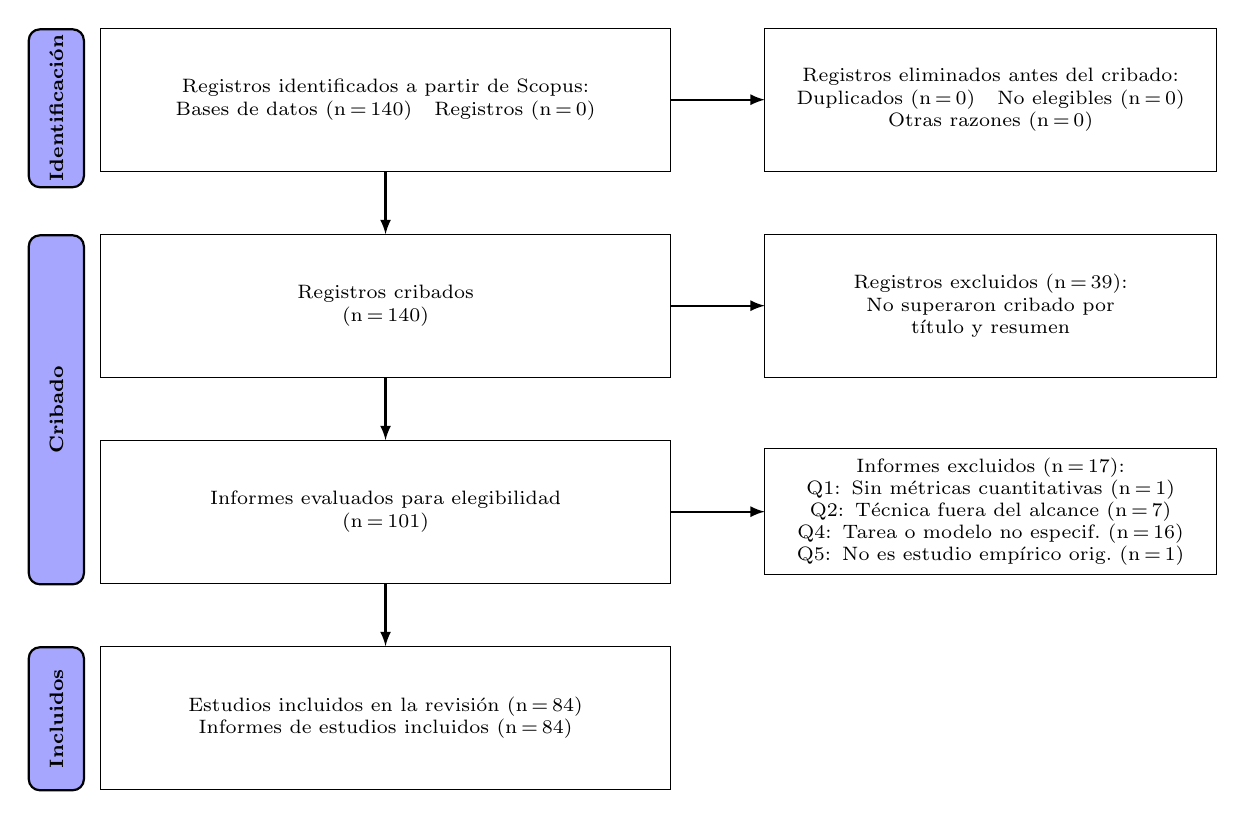
\begin{tikzpicture}[node distance=8mm and 12mm, start chain=going below,
    arrow/.style={-latex, thick},
    every node/.style={font=\scriptsize}]
\node[draw, rectangle, align=center, minimum height=12ex,
      text width=7cm, outer sep=0pt,
      on chain] (ident)
    {Registros identificados a partir de Scopus:\\
     Bases de datos (n\,=\,140)\quad Registros (n\,=\,0)};
\node[draw, rectangle, align=center, minimum height=12ex,
      text width=7cm, outer sep=0pt, on chain] (crib)
    {Registros cribados\\ (n\,=\,140)};
\node[draw, rectangle, align=center, minimum height=12ex,
      text width=7cm, outer sep=0pt, on chain] (eleg)
    {Informes evaluados para elegibilidad\\ (n\,=\,101)};
\node[draw, rectangle, align=center, minimum height=12ex,
      text width=7cm, outer sep=0pt, on chain] (incl)
    {Estudios incluidos en la revisión (n\,=\,84)\\
     Informes de estudios incluidos (n\,=\,84)};
\draw[arrow] (ident.south) -- (crib.north);
\draw[arrow] (crib.south)  -- (eleg.north);
\draw[arrow] (eleg.south)  -- (incl.north);
\node[draw, rectangle, align=center, minimum height=12ex,
      text width=5.5cm, outer sep=0pt,
      right=12mm of ident] (eprev)
    {Registros eliminados antes del cribado:\\
     Duplicados (n\,=\,0)\quad No elegibles (n\,=\,0)\\
     Otras razones (n\,=\,0)};
\node[draw, rectangle, align=center, minimum height=12ex,
      text width=5.5cm, outer sep=0pt,
      right=12mm of crib] (excl1)
    {Registros excluidos (n\,=\,39):\\
     No superaron cribado por\\
     título y resumen};
\node[draw, rectangle, align=center,
      text width=5.5cm, outer sep=0pt,
      right=12mm of eleg] (excl2)
    {Informes excluidos (n\,=\,17):\\
     Q1: Sin métricas cuantitativas (n\,=\,1)\\
     Q2: Técnica fuera del alcance (n\,=\,7)\\
     Q4: Tarea o modelo no especif.\ (n\,=\,16)\\
     Q5: No es estudio empírico orig.\ (n\,=\,1)};
\draw[arrow] (ident.east) -- (eprev.west);
\draw[arrow] (crib.east)  -- (excl1.west);
\draw[arrow] (eleg.east)  -- (excl2.west);
\path let \p1=(ident.north), \p2=(ident.south)
in node[draw, rounded corners, fill=blue!35, thick,
        inner sep=2pt, minimum width=7mm, minimum height={\y1-\y2},
        align=center, anchor=north east] at ([xshift=-2mm]ident.north west)
   {\rotatebox{90}{\textbf{\scriptsize Identificación}}};
\path let \p1=(crib.north), \p2=(eleg.south)
in node[draw, rounded corners, fill=blue!35, thick,
        inner sep=2pt, minimum width=7mm, minimum height={\y1-\y2},
        align=center, anchor=north east] at ([xshift=-2mm]crib.north west)
   {\rotatebox{90}{\textbf{\scriptsize Cribado}}};
\path let \p1=(incl.north), \p2=(incl.south)
in node[draw, rounded corners, fill=blue!35, thick,
        inner sep=2pt, minimum width=7mm, minimum height={\y1-\y2},
        align=center, anchor=north east] at ([xshift=-2mm]incl.north west)
   {\rotatebox{90}{\textbf{\scriptsize Incluidos}}};
\end{tikzpicture}%
}
\begin{flushleft}
\footnotesize
\textit{Nota.} Elaborado siguiendo las directrices de \textcite{page2021prisma}.
\end{flushleft}
\end{figure}

\subsection{Fase 1: Cribado de título y resumen}

Los 140 registros identificados en Scopus fueron evaluados mediante un sistema automatizado de votación por mayoría implementado con GPT-4o-mini. Cada registro recibió cuatro evaluaciones independientes, cada una con un perfil de evaluador distinto: experto en revisiones sistemáticas de NLP, revisor académico senior especializado en LLMs, investigador en aprendizaje automático, y experto en evaluación metodológica. La variación de perfiles buscó reducir sesgos al forzar perspectivas independientes sobre el mismo registro.

Cada evaluador respondió de manera binaria si el registro cumplía simultáneamente los tres criterios de inclusión:

\begin{itemize}
    \item \textbf{C1}: El artículo trata sobre \textit{fine-tuning} de \textit{Large Language Models} (GPT, LLaMA, Mistral, Claude, Falcon, BLOOM, OPT). Se excluyen modelos \textit{encoder-only} como BERT o RoBERTa.
    \item \textbf{C2}: El artículo evalúa al menos una de las nueve técnicas objetivo: \textit{Full Fine-Tuning}, SFT, LoRA, QLoRA, \textit{Adapter Layers}, \textit{Prefix Tuning}, \textit{Prompt Tuning}, RLHF o DPO.
    \item \textbf{C3}: El artículo reporta evaluación empírica con métricas cuantitativas (\textit{accuracy}, F1, BLEU, ROUGE, \textit{perplexity} o \textit{benchmark scores}).
\end{itemize}

La decisión final se determinó por mayoría simple: con tres o más votos favorables el registro fue aceptado, con dos o menos fue rechazado. Los registros con empate exacto fueron marcados para revisión manual. De los 140 registros evaluados, 101 superaron esta fase y avanzaron a la evaluación de texto completo. Los 39 registros restantes fueron excluidos por no cumplir los criterios de inclusión.

\subsection{Fase 2: Evaluación de texto completo}

Los 101 artículos fueron evaluados en texto completo mediante Claude Sonnet 4.6, utilizando \textit{tool use} estructurado para garantizar respuestas en formato JSON validado. El texto completo de cada PDF fue extraído automáticamente mediante PyMuPDF y enviado al modelo junto con cinco criterios de elegibilidad:

\begin{itemize}
    \item \textbf{Q1}: ¿El artículo reporta resultados numéricos explícitos usando \textit{accuracy}, F1, \textit{precision}, \textit{recall}, BLEU, ROUGE u otros \textit{scores} de \textit{benchmarks} estándar?
    \item \textbf{Q2}: ¿El artículo implementa al menos una técnica en scope con evidencia de aplicación real, reportando \textit{optimizer}, \textit{dataset} y \textit{training steps} o \textit{epochs}?
    \item \textbf{Q3}: ¿El artículo identifica el \textit{dataset} utilizado especificando nombre y dominio de aplicación?
    \item \textbf{Q4}: ¿El artículo especifica tanto la tarea NLP realizada como la arquitectura del modelo base utilizado?
    \item \textbf{Q5}: ¿Es un estudio empírico original con resultados experimentales propios, excluyendo \textit{surveys}, revisiones de literatura y artículos teóricos?
\end{itemize}

Los criterios Q1, Q2, Q4 y Q5 operaron con lógica eliminatoria directa: un resultado negativo en cualquiera resultó en exclusión inmediata. El criterio Q3 recibió tratamiento especial: un resultado negativo derivó en revisión manual en lugar de exclusión directa, dado que estudios de dominio aplicado pueden describir correctamente su corpus sin nombrar un \textit{dataset} público estándar. De los 101 artículos evaluados, 84 fueron incluidos y 17 excluidos. La Figura~\ref{fig:criterios} desglosa las exclusiones por criterio, evidenciando que Q4 fue el más restrictivo con 16 exclusiones, seguido de Q2 con 7. Los criterios Q1 y Q5 generaron una exclusión cada uno, mientras que Q3 no produjo exclusiones directas dado que los casos negativos derivaron en revisión manual.

\begin{figure}[H]
    \centering
    \caption{Artículos excluidos por cada criterio de elegibilidad en la Fase 2 (n = 101)}
    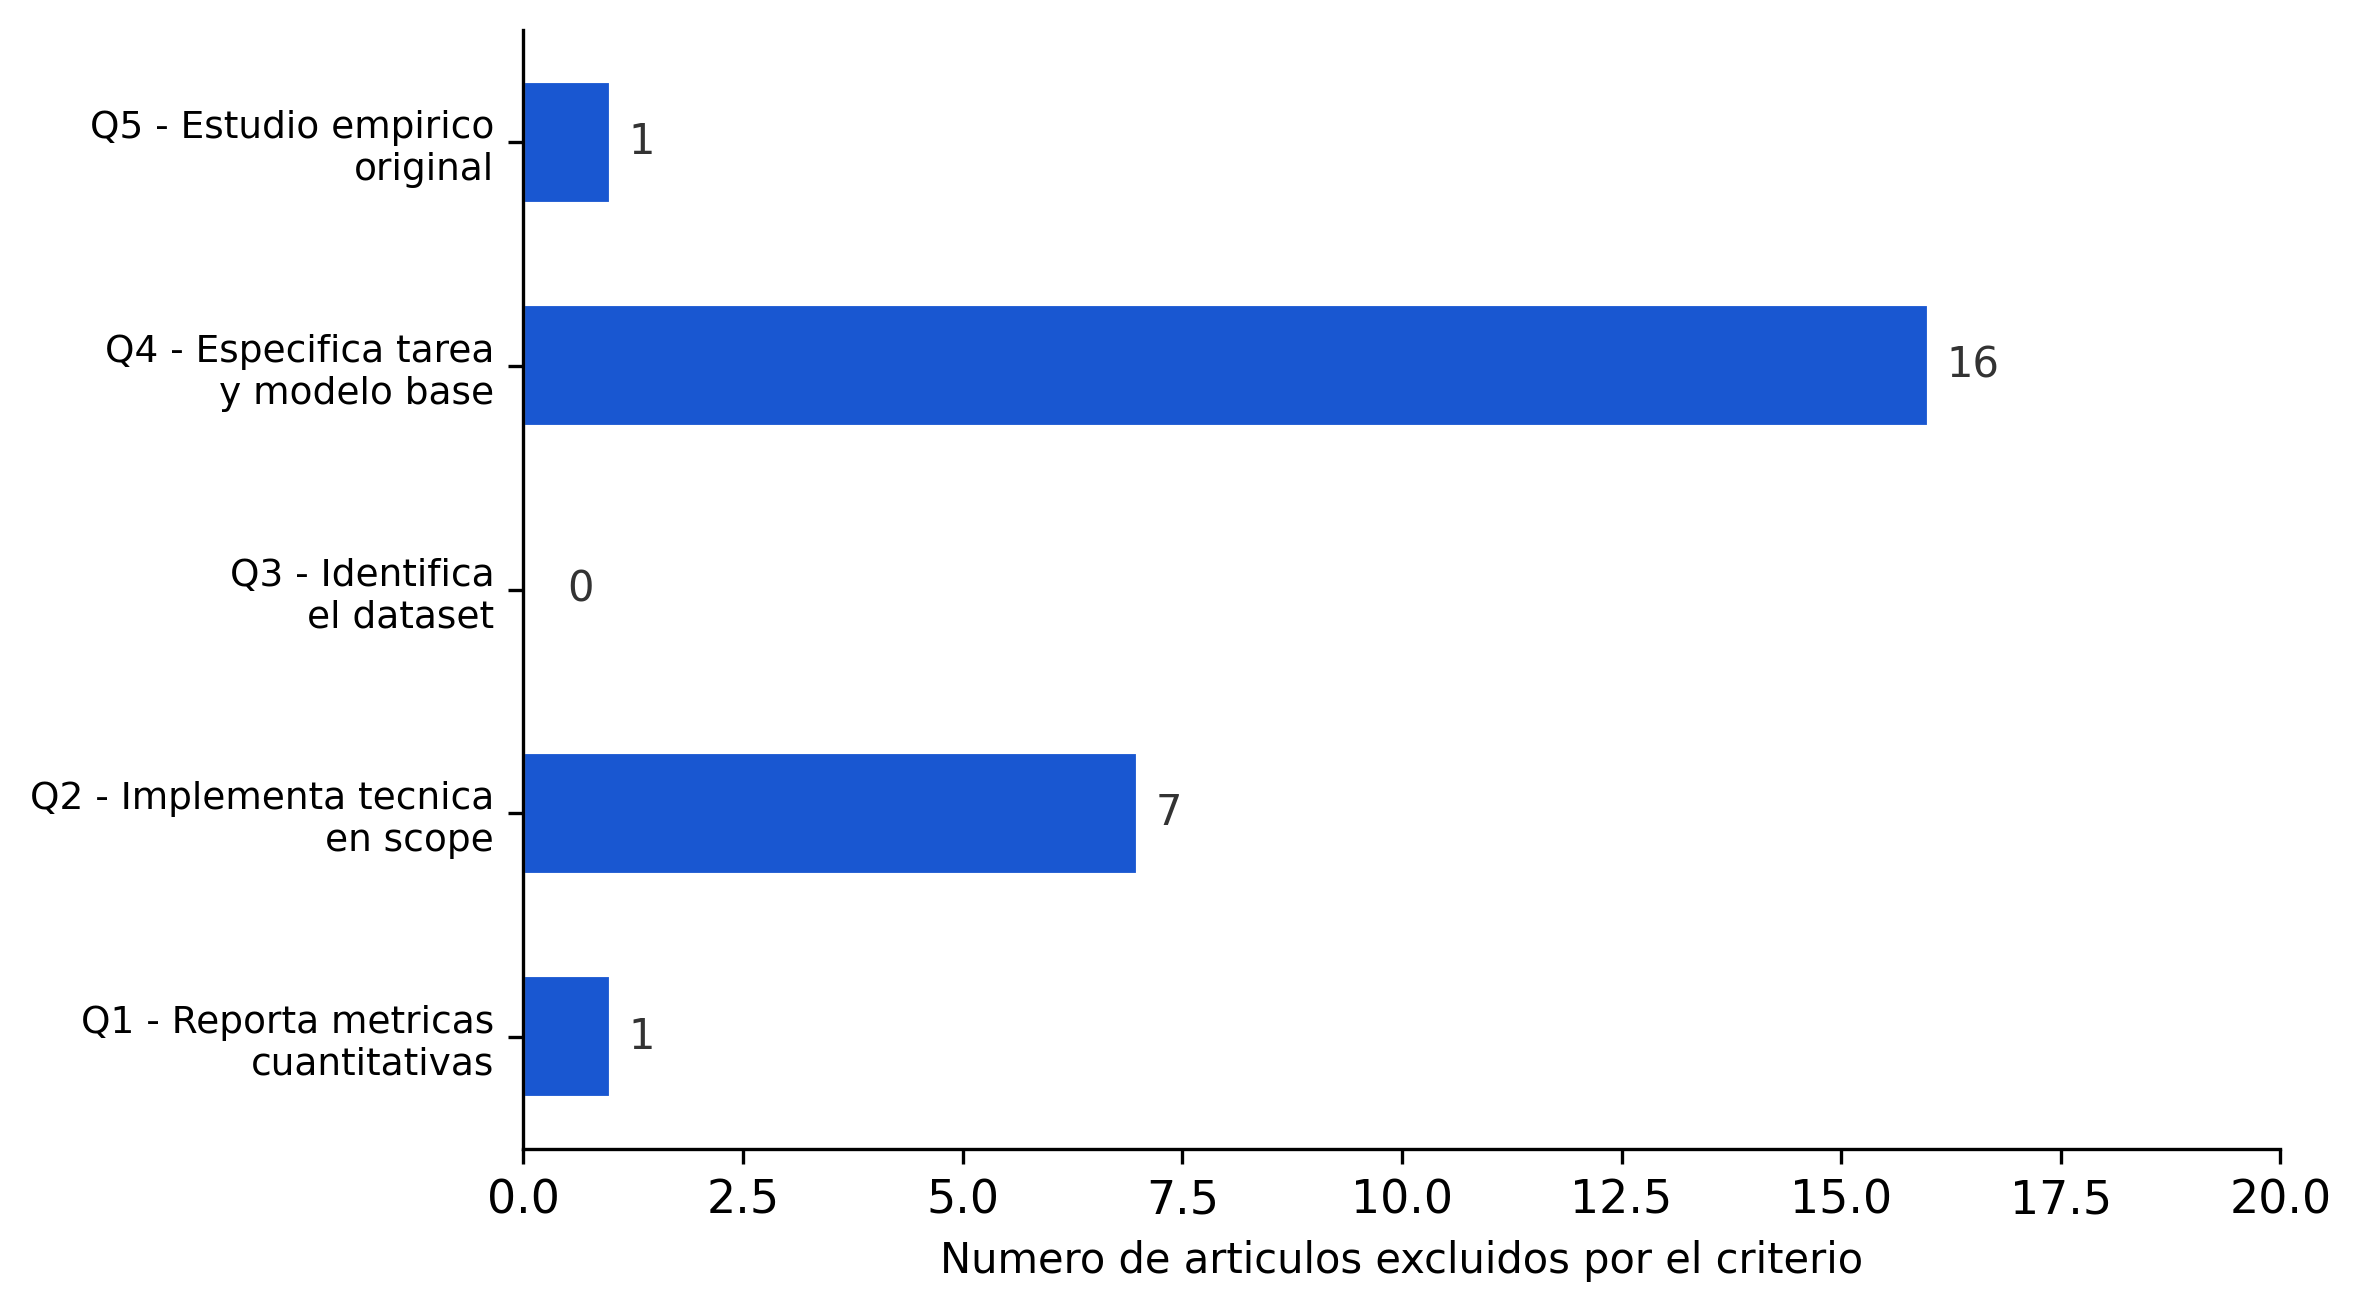
\includegraphics[width=0.85\linewidth]{Imagenes/fig1_criterios_elegibilidad.png}
    \label{fig:criterios}
    \begin{flushleft}
    \footnotesize
    \textit{Nota.} El criterio Q3 no aparece con exclusiones directas porque los casos negativos derivaron en revisión manual. Los valores pueden sumar más de 17 si un mismo artículo no cumplió más de un criterio.
    \end{flushleft}
\end{figure}

%%%%%%%%%%%%%%%%%%%%%%%%%%%%%%%%%%%%%%%%
\section{Evaluación de calidad metodológica}

Los 84 estudios incluidos fueron sometidos a una evaluación de calidad metodológica mediante Claude Haiku 4.5, utilizando \textit{tool use} estructurado sobre el texto completo de cada artículo. Cada estudio fue evaluado según tres criterios en escala 0\,/\,0.5\,/\,1, con un score máximo de 3,0:

\begin{itemize}
    \item \textbf{QA1}: ¿El artículo reporta explícitamente las proporciones del \textit{split} train/test o los tamaños exactos de cada subconjunto?
    \item \textbf{QA3}: ¿El artículo reporta una configuración de entrenamiento completa incluyendo \textit{learning rate}, \textit{batch size}, \textit{epochs} y parámetros técnica-específicos?
    \item \textbf{QA4}: ¿El artículo caracteriza completamente el \textit{dataset} con nombre, dominio y tamaño?
\end{itemize}

Los scores obtenidos en esta evaluación se emplean como criterio de priorización interpretativa en la síntesis comparativa presentada en el capítulo de Resultados: los hallazgos provenientes de estudios con score alto (score $\geq$ 2,5) se priorizaron como soporte principal de los patrones transversales identificados, mientras que los hallazgos de estudios con calidad media se reportan en el análisis descriptivo pero no fundamentan las conclusiones comparativas.

%%%%%%%%%%%%%%%%%%%%%%%%%%%%%%%%%%%%%%%%
\section{Clasificación por dominio de aplicación}

Cada uno de los 84 estudios incluidos fue asignado a uno de cuatro dominios de aplicación definidos a priori. La clasificación se realizó de forma automatizada durante la Fase 3, como parte del mismo proceso de evaluación de calidad metodológica, utilizando el texto completo de cada artículo como insumo. Los criterios de asignación empleados fueron los siguientes:

\begin{itemize}
    \item \textbf{Salud y Biomedicina}: estudios cuya tarea principal involucra NLP clínico, registros médicos, texto biomédico, descubrimiento de fármacos, salud mental, radiología, genómica o datos de pacientes.
    \item \textbf{Ciencias Exactas y Computación}: estudios enfocados en generación de código, razonamiento matemático, ingeniería de software, verificación formal, tareas de programación, ciberseguridad o \textit{benchmarks} de ciencias de la computación.
    \item \textbf{Lenguaje y Humanidades}: estudios que abordan tareas generales de NLP como traducción, resumen, análisis de sentimiento, reconocimiento de entidades nombradas, respuesta a preguntas sobre corpus generales, lingüística, literatura o texto de redes sociales.
    \item \textbf{Industria y Negocios}: estudios con aplicaciones en finanzas, derecho, educación, atención al cliente, comercio electrónico, recursos humanos, logística o aplicaciones empresariales.
\end{itemize}

Cuando un estudio evaluaba múltiples tareas en dominios distintos, se asignó al dominio principal según la contribución declarada por los autores. Esta clasificación constituye el eje organizador del análisis comparativo presentado en el capítulo de Resultados.

%%%%%%%%%%%%%%%%%%%%%%%%%%%%%%%%%%%%%%%%
\section{Extracción de datos}

De cada uno de los 84 estudios incluidos en el corpus final se extrajeron datos estructurados mediante lectura directa del texto completo de cada artículo. Este proceso se realizó de forma independiente al pipeline de selección PRISMA descrito en las secciones anteriores. Como apoyo a la identificación inicial, se empleó un modelo de lenguaje (Claude, Anthropic) para localizar en cada artículo la técnica principal implementada, la tarea de aplicación y la presencia o ausencia de un \textit{baseline} de referencia explícito; los valores finales fueron verificados y registrados manualmente contrastando cada campo contra el texto original del artículo.

Los campos extraídos fueron los siguientes: técnica de \textit{fine-tuning} implementada, tarea y dominio de aplicación, métrica principal de evaluación, valor del \textit{baseline} de referencia y mejor resultado obtenido por el modelo evaluado. A partir de los dos últimos campos se calculó el incremento porcentual ($\Delta$\%) respecto al \textit{baseline}. Los campos no reportados explícitamente en el artículo fueron registrados como \textit{not reported}, sin inferencia ni estimación de valores ausentes.

Para que el cálculo de mejora relativa fuera metodológicamente válido, se aplicó un criterio de comparabilidad: un estudio se consideró comparable únicamente si los autores declaraban un \textit{baseline} único y explícito contra el cual comparar el resultado principal. Quedaron excluidos de la comparación cuantitativa los estudios que evaluaban múltiples modelos sin designar una referencia de comparación fija, y aquellos donde se presentaban resultados para más de un modelo \textit{fine-tuneado} sin indicar cuál constituía el resultado principal, impidiendo el cálculo de un incremento atribuible a la técnica de forma aislada. Bajo este criterio, 30 de los 84 estudios presentaron pares de valores comparables; los 54 restantes se reportan en el análisis descriptivo del corpus pero no contribuyen a la síntesis cuantitativa de mejora relativa.

%%%%%%%%%%%%%%%%%%%%%%%%%%%%%%%%%%%%%%%%
\section{Análisis de datos}

El análisis de datos se organizó en tres niveles complementarios sobre el corpus de 84 estudios incluidos.

El análisis descriptivo caracterizó el corpus mediante frecuencias de técnicas de \textit{fine-tuning}, distribución por dominio de aplicación, modelos base más utilizados y métricas de evaluación más frecuentes. Este nivel permitió identificar los patrones dominantes en la literatura reciente sobre \textit{fine-tuning} de LLMs.

El análisis comparativo sintetizó el rendimiento reportado por dominio de aplicación, comparando los resultados de cada estudio contra sus \textit{baselines} de referencia dentro de cada dominio. Dado que los estudios emplean métricas y \textit{datasets} heterogéneos, la comparación se realizó a nivel de mejora relativa sobre el \textit{baseline} en lugar de valores absolutos, permitiendo identificar patrones de efectividad por dominio independientes de la escala de cada métrica.

El análisis de calidad metodológica empleó los \textit{scores} obtenidos en la evaluación de calidad como criterio de priorización interpretativa: los hallazgos provenientes de estudios con \textit{score} alto (\textit{score} $\geq$ 2,5) se priorizaron como soporte principal de los patrones transversales identificados, mientras que los hallazgos de estudios con calidad media se reportan en el análisis descriptivo pero no fundamentan las conclusiones comparativas.
%%%%%%%%%%%%%%%%%%%%%%%%%%%%%%%%%%%%%%%%
\chapter{Resultados y discusión}
%%%%%%%%%%%%%%%%%%%%%%%%%%%%%%%%%%%%%%%%

%%%%%%%%%%%%%%%%%%%%%%%%%%%%%%%%%%%%%%%%
\section{Caracterización del corpus}

El proceso de selección PRISMA resultó en la inclusión de 84 estudios a partir de 140 registros identificados en Scopus. Las exclusiones en la Fase 2 correspondieron principalmente a artículos que no especificaban la tarea NLP ni el modelo base (Q4, n~=~16), con casos como predicción de trayectorias, clasificación de señales de sensores y regresión numérica sobre datos tabulares, seguido de técnicas fuera del alcance del estudio (Q2, n~=~7) y ausencia de resultados experimentales propios (Q5, n~=~1).

La clasificación de los 84 estudios en cuatro dominios de aplicación se realizó de forma automatizada durante la Fase 3, aplicando los criterios definidos en la sección de Metodología. La distribución resultante evidencia un marcado predominio del área de Salud y Biomedicina, con 30 estudios (35,7\%), seguido de Lenguaje y Humanidades con 21 (25,0\%), Ciencias Exactas y Computación con 20 (23,8\%) e Industria y Negocios con 13 (15,5\%). Esta distribución refleja la intensa actividad investigativa que el \textit{fine-tuning} de \textit{Large Language Models} ha tenido en aplicaciones clínicas y biomédicas durante el período 2020--2025, fenómeno concordante con la disponibilidad de corpus especializados como PubMed y MIMIC y con la demanda de modelos adaptados para tareas de extracción de información médica. La Figura~\ref{fig:dominios} presenta esta distribución de forma visual.

\begin{figure}[H]
    \centering
    \caption{Distribución del corpus por dominio de aplicación (n = 84)}
    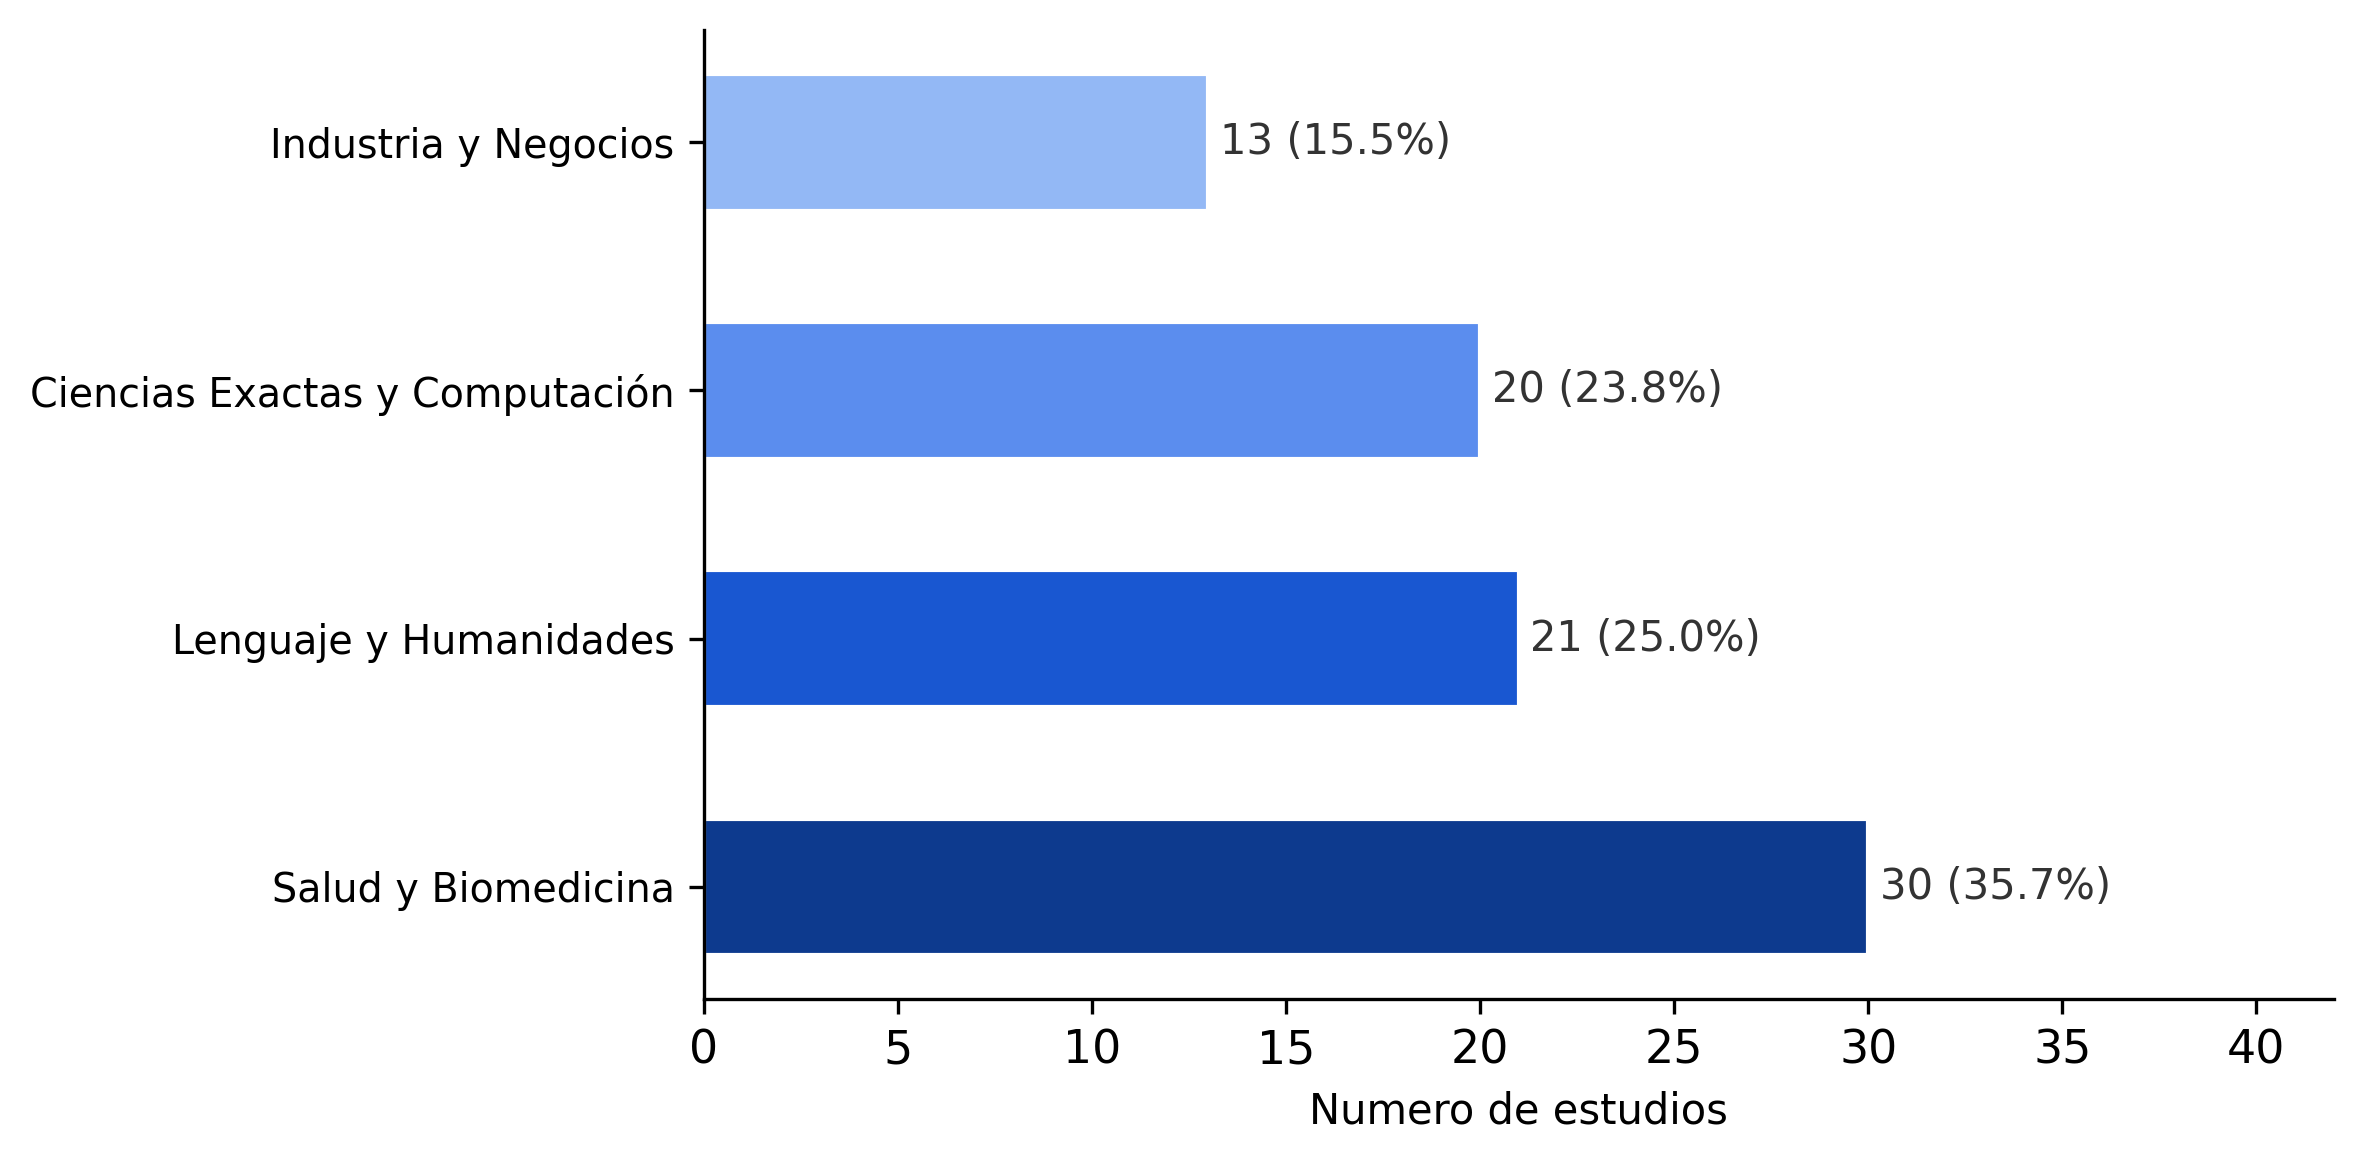
\includegraphics[width=0.85\linewidth]{Imagenes/fig2_distribucion_dominios.png}
    \label{fig:dominios}
\end{figure}

La calidad metodológica del corpus fue aceptable en conjunto: el \textit{score} promedio fue de 2,61 sobre 3,0, con la mayoría de estudios por encima del umbral de priorización de 2,5 establecido en la Metodología. A nivel de criterios individuales, QA4 obtuvo la puntuación media más alta, reflejando que prácticamente la totalidad de los estudios caracteriza con precisión sus \textit{datasets}. QA1 y QA3 presentaron medias más bajas, con una proporción menor de estudios que reportan \textit{splits} explícitos o que detallan de forma completa los hiperparámetros de entrenamiento. Por dominio, Lenguaje y Humanidades concentra la mayor calidad metodológica promedio, mientras que Industria y Negocios presenta la media más baja con la mayor variabilidad, lo que refleja heterogeneidad en las prácticas de reporte dentro de ese dominio.

%%%%%%%%%%%%%%%%%%%%%%%%%%%%%%%%%%%%%%%%
\section{Resultados por dominio}

%%%%%%%%%%%%%%%%%%%%%%%%%%%%%%%%%%%%%%%%
\subsection{Salud y Biomedicina}

El dominio de Salud y Biomedicina concentra 30 estudios, constituyendo el grupo más numeroso del corpus (35,7\%).

\subsubsection{Técnicas y modelos predominantes}

En este dominio, LoRA y QLoRA constituyen la categoría dominante con 21 de los 30 estudios (70,0\%), seguidas de técnicas alternativas como Adapters, Prefix Tuning y variantes con 5 estudios (16,7\%), \textit{Full Fine-Tuning} con 3 (10,0\%) y métodos de alineación con 1 (3,3\%). Dentro de la familia LoRA, dos estudios incorporan GRPO como mecanismo de alineación: educación cardiovascular \parencite{rullo2025cardio} y generación de reportes clínicos \parencite{kuo2025medical}. El único método de alineación es SFT+DPO para razonamiento clínico \parencite{savage2025dpo}. Técnicas alternativas como P-Tuning v2 \parencite{liu2024cpmi} y \textit{Prompt Tuning} \parencite{yang2025ceprompt} aparecen de forma puntual, reflejando que el dominio biomédico experimenta con distintos enfoques de adaptación paramétrica aunque LoRA concentra la mayoría de las aplicaciones.

\subsubsection{Tareas y métricas}

Las tareas identificadas en el dominio se agrupan en cuatro categorías principales. La extracción de información clínica (reconocimiento de entidades nombradas, extracción de medicamentos y relaciones) es la más frecuente, con estudios en NER médico en chino \parencite{zhou2024adapter} y extracción de medicamentos \parencite{richterpechanski2025medication}. Le siguen la respuesta a preguntas médicas y los sistemas de diálogo especializado \parencite{adhikary2025medical, bayram2025medical, tong2025xuanhugpt}, la generación y resumen de texto clínico \parencite{chao2025evaluating, hou2024ft} y la clasificación en salud pública, que abarca análisis de sentimiento \parencite{elmitwalli2024ft} y detección de desinformación \parencite{zhao2025daft}.

La heterogeneidad de métricas reportadas refleja directamente la diversidad de subtareas. En tareas de extracción y clasificación predominan F1 y sus variantes; en NER médico, por ejemplo, se reporta una mejora de F1 de 62,40\% a 65,90\% \parencite{zhou2024adapter}. En tareas de generación y resumen predominan ROUGE y BLEU, con ejemplos como la generación de cartas médicas \parencite{hou2024ft}. Una limitación recurrente en el corpus es la ausencia de un \textit{baseline} declarado explícitamente: varios estudios evalúan múltiples modelos o configuraciones y reportan el mejor resultado sin establecer una referencia de comparación fija, lo que impide atribuir la mejora a la técnica de \textit{fine-tuning} de forma aislada. De los 30 estudios, 9 reportan métricas cuantitativas comparables; los resultados detallados por estudio se presentan en la Tabla~\ref{tab:apx_salud} del Apéndice~A.

\subsubsection{Patrones de aplicabilidad}

Del análisis de los 30 estudios emergen tres patrones de aplicabilidad consistentes en el dominio.

El primero es la ventaja del \textit{fine-tuning} específico sobre el modelo base sin adaptar. Los estudios con resultados numéricos explícitos muestran que LoRA y QLoRA producen mejoras sustanciales sobre los \textit{baselines} de referencia en las subtareas evaluadas. Este patrón se observa en el dominio geriátrico, donde LLaMA3.1-8B ajustado sobre datos de cuidado especializado mejora de ROUGE 8,60\% a 34,96\% (+306,5\%) respecto al mismo modelo sin adaptar \parencite{xu2025cpel}, y en generación de cartas médicas, donde QLoRA mejora ROUGE-1 de 0,161 a 0,352 (+118,6\%) \parencite{hou2024ft}.

El segundo es la preferencia por modelos abiertos en entornos regulados. La imposibilidad de enviar datos clínicos sensibles a APIs externas condiciona directamente la elección de técnica y arquitectura. Al menos un estudio señala explícitamente que los modelos propietarios no pudieron ser evaluados porque las versiones seguras para datos clínicos protegidos no estaban disponibles al momento del estudio \parencite{chao2025evaluating}. Este condicionante favorece el despliegue local mediante técnicas como QLoRA o LoRA estándar, que no requieren dependencia de servicios externos.

El tercero es la efectividad de LoRA en lenguas con escasa representación en los corpus de preentrenamiento. En idiomas como turco, vietnamita y árabe médico, donde los modelos base tienen menor exposición previa, LoRA produce adaptaciones consistentes al dominio clínico \parencite{bayram2025medical, bui2025ft, khader2025ft}. El mismo comportamiento se observa en dominios de conocimiento altamente especializado como la medicina tradicional china \parencite{yang2024tcmgpt, tong2025xuanhugpt}.

%%%%%%%%%%%%%%%%%%%%%%%%%%%%%%%%%%%%%%%%
\subsection{Lenguaje y Humanidades}

El dominio de Lenguaje y Humanidades concentra 21 estudios (25,0\%) y presenta la mayor calidad metodológica promedio entre los cuatro dominios.

\subsubsection{Técnicas y modelos predominantes}

LoRA y QLoRA constituyen también la categoría dominante con 16 de los 21 estudios (76,2\%), seguidas de técnicas alternativas como \textit{Adapter Layers} \parencite{chen2025adaptforever}, Multi-PEFT \parencite{jia2025agnostic} y \textit{Prompt Tuning} \parencite{cheng2025prompt} con 3 estudios (14,3\%), y métodos de alineación con 2 (9,5\%): DPO para Q\&A en kazajo \parencite{kadyrbek2025dpo} y ORPO para análisis de sentimiento \parencite{shen2025ft}. Esta distribución refleja mayor diversidad metodológica que otros dominios del corpus.

\subsubsection{Tareas y métricas}

Las tareas en este dominio son heterogéneas y reflejan la amplitud del área. Las más frecuentes son análisis de sentimiento y detección de lenguaje ofensivo \parencite{shen2025ft, wang2025lora, zain2025ruold, rathore2025ft}, seguidas de respuesta a preguntas y razonamiento \parencite{chen2025ft, li2025keft, cheng2025prompt}. Otras tareas identificadas son traducción automática y estimación de calidad \parencite{khoboko2025ft, sindhujan2025translation} y evaluación educativa automatizada \parencite{anghel2025courseeval}.

Las métricas varían según la subtarea. F1 y \textit{accuracy} predominan en clasificación; en lenguaje ofensivo, por ejemplo, se reporta una mejora de Macro-F1 de 80,1 a 81,3 (+1,5\%) \parencite{wang2025lora}. En respuesta a preguntas predominan métricas de solapamiento como ROUGE-L, con una mejora de 22,39\% a 47,85\% (+113,7\%) en Q\&A sobre patrimonio cultural \parencite{chen2025ft}. De los 21 estudios, 9 reportan métricas cuantitativas comparables; los resultados detallados por estudio se presentan en la Tabla~\ref{tab:apx_lh} del Apéndice~A.

\subsubsection{Patrones de aplicabilidad}

Del análisis de los 21 estudios emergen dos patrones de aplicabilidad predominantes en el dominio.

El primero es la efectividad de las técnicas de \textit{fine-tuning} eficiente en lenguas de bajos recursos y dominios culturalmente específicos. Varios estudios demuestran que LoRA, QLoRA y métodos de alineación como DPO permiten adaptar modelos generales a lenguas con escasa representación en los datos de preentrenamiento, como kazajo y zulú, con mejoras consistentes sobre los \textit{baselines} \parencite{kadyrbek2025dpo, khoboko2025ft}. Este patrón refuerza la aplicabilidad transversal de las técnicas PEFT en escenarios de recursos limitados y complementa lo observado en Salud y Biomedicina con lenguas como turco, vietnamita y árabe.

El segundo es la diversificación de enfoques PEFT orientados a tareas específicas. La aparición de Multi-PEFT, \textit{Adapter Layers}, \textit{Prompt Tuning} y métodos de alineación como ORPO en este dominio sugiere que la investigación en Lenguaje y Humanidades está explorando combinaciones y variantes más allá de LoRA estándar. Arquitecturas agnósticas a la tarea que combinan múltiples estrategias PEFT superan a LoRA estándar en \textit{benchmarks} de clasificación y razonamiento, con una mejora de Macro-F1 de 0,8712 a 0,8736 sobre el mejor \textit{baseline} disponible \parencite{jia2025agnostic}, y Adapter Layers mejoran el rendimiento promedio en clasificación GLUE de 86,4 a 89,0 (+3,0\%) \parencite{chen2025adaptforever}.

%%%%%%%%%%%%%%%%%%%%%%%%%%%%%%%%%%%%%%%%
\subsection{Ciencias Exactas y Computación}

El dominio de Ciencias Exactas y Computación concentra 20 estudios (23,8\%).

\subsubsection{Técnicas y modelos predominantes}

LoRA y QLoRA alcanzan en este dominio su mayor concentración relativa del corpus, con 17 de los 20 estudios (85,0\%), incluyendo combinaciones como LoRA+RLHF \parencite{gorbatovski2024qa} y DP-LoRA \parencite{liu2025federated}. Las técnicas alternativas (Prefix Tuning, \textit{Prompt Tuning} y combinaciones múltiples) representan 3 estudios (15,0\%) \parencite{jung2025prefix, prottasha2024peft, zou2025peft}.

\subsubsection{Tareas y métricas}

Las tareas se agrupan en tres categorías principales. La más frecuente es el razonamiento y la respuesta a preguntas sobre \textit{benchmarks} de propósito general, presente en estudios que evalúan técnicas sobre conjuntos como SuperGLUE \parencite{liu2025tasks}, GLUE \parencite{jung2025prefix} y razonamiento de sentido común \parencite{wang2025ft}. Le sigue la ingeniería de software, con estudios que abarcan resumen de reportes de bugs \parencite{xiang2024sumllama, choi2025agentreport}, generación de código \parencite{ulurmak2025ft} y razonamiento sobre grafos \parencite{chen2025glr}. El aprendizaje federado con técnicas PEFT aparece en cuatro estudios \parencite{elbakary2025mira, li2025federated, liu2025federated, iftikhar2025peft}, reflejando un interés creciente en la adaptación de modelos bajo restricciones de privacidad distribuida.

Las métricas más frecuentes son \textit{accuracy} y sus variantes en tareas de razonamiento \parencite{liu2025tasks, iftikhar2025peft}. ROUGE predomina en tareas de generación y resumen; en resumen de reportes de bugs, por ejemplo, se reportan mejoras de ROUGE-1 Recall de 61,0\% a 84,6\% (+38,7\%) \parencite{choi2025agentreport} y de ROUGE-L de 39,69 a 41,01 (+3,3\%) \parencite{xiang2024sumllama}. De los 20 estudios, 6 reportan \textit{baseline} explícito que permite calcular mejora relativa, mientras que 14 no incluyen referencia de comparación directa; los resultados detallados por estudio se presentan en la Tabla~\ref{tab:apx_cec} del Apéndice~A.

\subsubsection{Patrones de aplicabilidad}

Del análisis de los 20 estudios emergen dos patrones de aplicabilidad en el dominio.

El primero es la adopción transversal de LoRA y QLoRA en tareas computacionales de distinta naturaleza. La concentración en 17 de los 20 estudios refleja que esta familia de técnicas se aplica de forma consistente tanto en tareas de razonamiento sobre \textit{benchmarks} como en ingeniería de software. Entre los estudios con métricas comparables, las mejoras van desde incrementos moderados en resumen de reportes de bugs \parencite{xiang2024sumllama} hasta ganancias pronunciadas en entrenamiento multi-parte, donde LoRA mejora \textit{accuracy} de 14,25 a 65,43 (+359,2\%) \parencite{liu2025mpctf}, lo que sugiere que la técnica se adapta a contextos experimentales diversos dentro del dominio.

El segundo es la aplicación de técnicas PEFT en escenarios de aprendizaje federado como dirección de investigación emergente. Cuatro estudios exploran la combinación de LoRA con marcos de aprendizaje federado para entrenar modelos sobre datos distribuidos sin centralización \parencite{elbakary2025mira, li2025federated, liu2025federated, iftikhar2025peft}. Los resultados disponibles son mixtos: un estudio reporta una mejora de \textit{accuracy} de 71,2\% a 73,8\% \parencite{iftikhar2025peft} mientras que otro muestra una leve caída de 76,6\% a 75,4\% \parencite{li2025federated}, lo que indica que esta combinación está aún en fase exploratoria sin evidencia consolidada de efectividad.

%%%%%%%%%%%%%%%%%%%%%%%%%%%%%%%%%%%%%%%%
\subsection{Industria y Negocios}

El dominio de Industria y Negocios concentra 13 estudios (15,5\%), siendo el grupo menos numeroso del corpus. La calidad metodológica promedio es la más baja de los cuatro dominios y con la mayor variabilidad, lo que refleja heterogeneidad en las prácticas de reporte dentro del dominio.

\subsubsection{Técnicas y modelos predominantes}

LoRA o alguna de sus variantes aparece en los 13 estudios del dominio (100,0\%), confirmando su posición como categoría predominante. Varios estudios combinan LoRA con técnicas complementarias: con RLHF para generación de patentes \parencite{ren2025patent} y con RAG para Q\&A sobre protección fitosanitaria \parencite{xiong2025lora}. La variante MoELoRA se aplica a mantenimiento minero \parencite{cao2025lora}, y LoRA combinada con RLHF-PPO a generación de texto legal \parencite{peng2025keyword}.

\subsubsection{Tareas y métricas}

Las tareas son aplicadas y de nicho específico. Las más frecuentes son la generación de texto especializado en dominios verticales, con estudios que abarcan generación de patentes \parencite{ren2025patent}, análisis de riesgo en mantenimiento minero \parencite{cao2025lora, sun2024mirachatglm}, consultoría en acuicultura \parencite{song2025lora} y generación de texto legal \parencite{peng2025keyword}. Le siguen sistemas de Q\&A y recuperación de información en dominios industriales \parencite{xiong2025lora, zhou2025kg}; a estos se suman análisis de sentimiento en redes sociales \parencite{lin2024lora} y extracción geoespacial \parencite{han2025ft2}.

Las métricas reportadas son heterogéneas: ROUGE-L en consultoría de dominio \parencite{song2025lora} y Macro-F1 en extracción de información \parencite{yang2025hierarchic}. De los 13 estudios, 6 reportan \textit{baseline} explícito que permite calcular mejora relativa; los resultados detallados por estudio se presentan en la Tabla~\ref{tab:apx_ib} del Apéndice~A.

\subsubsection{Patrones de aplicabilidad}

Del análisis de los 13 estudios emergen dos patrones de aplicabilidad característicos del dominio.

El primero es la combinación sistemática de LoRA con técnicas complementarias para tareas de generación de alto valor. En los estudios con resultados cuantitativos más destacados, LoRA no actúa sola sino combinada con RLHF como mecanismo de alineación o con RAG como fuente de conocimiento actualizado. La combinación LoRA+RLHF produce una mejora de BLEU-4 de 11,663 a 45,360 (+288,9\%) en escala 0-100 en generación de patentes \parencite{ren2025patent}, y LoRA+RAG mejora ROUGE-2 de 0,121 a 0,321 (+165,3\%) en Q\&A sobre protección fitosanitaria \parencite{xiong2025lora}. Este patrón sugiere que en aplicaciones industriales donde la calidad del texto generado es crítica, la combinación de LoRA con mecanismos complementarios es la configuración predominante.

El segundo es la aplicabilidad de LoRA en dominios de conocimiento altamente especializado. En acuicultura \parencite{song2025lora}, mantenimiento minero \parencite{cao2025lora} y gestión de emergencias \parencite{zhou2025kg}, LoRA produce mejoras consistentes en dominios verticales con vocabulario técnico específico y escasa representación en los corpus de preentrenamiento. En NER de emergencias, por ejemplo, se reporta una mejora de F1 de 0,7874 a 0,8920 (+13,3\%) \parencite{zhou2025kg}.

%%%%%%%%%%%%%%%%%%%%%%%%%%%%%%%%%%%%%%%%
\section{Análisis comparativo entre dominios}

El análisis transversal de los cuatro dominios permite identificar patrones globales en el uso de técnicas de \textit{fine-tuning}, la cobertura metodológica del corpus y las diferencias en rendimiento reportado entre contextos de aplicación.

%%%%%%%%%%%%%%%%%%%%%%%%%%%%%%%%%%%%%%%%
\subsection{Distribución de técnicas}

A nivel global, cualquier variante de LoRA o QLoRA aparece en 67 de los 84 estudios del corpus (79,8\%), consolidando esta categoría como la más adoptada independientemente del dominio. Le siguen otras técnicas PEFT sin LoRA ni QLoRA con 11 estudios (13,1\%), \textit{Full Fine-Tuning} e \textit{Instruction Tuning} con 3 (3,6\%) y métodos de alineación sin LoRA con 3 (3,6\%).

La familia PEFT emerge como dominante en todos los dominios del corpus, con LoRA como técnica principal. La concentración de LoRA/QLoRA crece progresivamente desde Salud y Biomedicina (70,0\%) hacia Industria y Negocios (100,0\%), lo que sugiere que cuanto más especializado y orientado a producción es el contexto, mayor es la convergencia hacia LoRA como técnica estándar. Los métodos de alineación mantienen una presencia marginal pero consistente en dos de los cuatro dominios, mientras que \textit{Full Fine-Tuning} y SFT quedan restringidos a los dominios con mayor demanda de adaptación completa del modelo.

La Figura~\ref{fig:familias} presenta la distribución por familia de técnicas en cada dominio, y la Figura~\ref{fig:tecnicas} desglosa las técnicas específicas identificadas en el corpus.

\begin{figure}[H]
    \centering
    \caption{Distribución por familia de técnicas de \textit{fine-tuning} por dominio (n = 84)}
    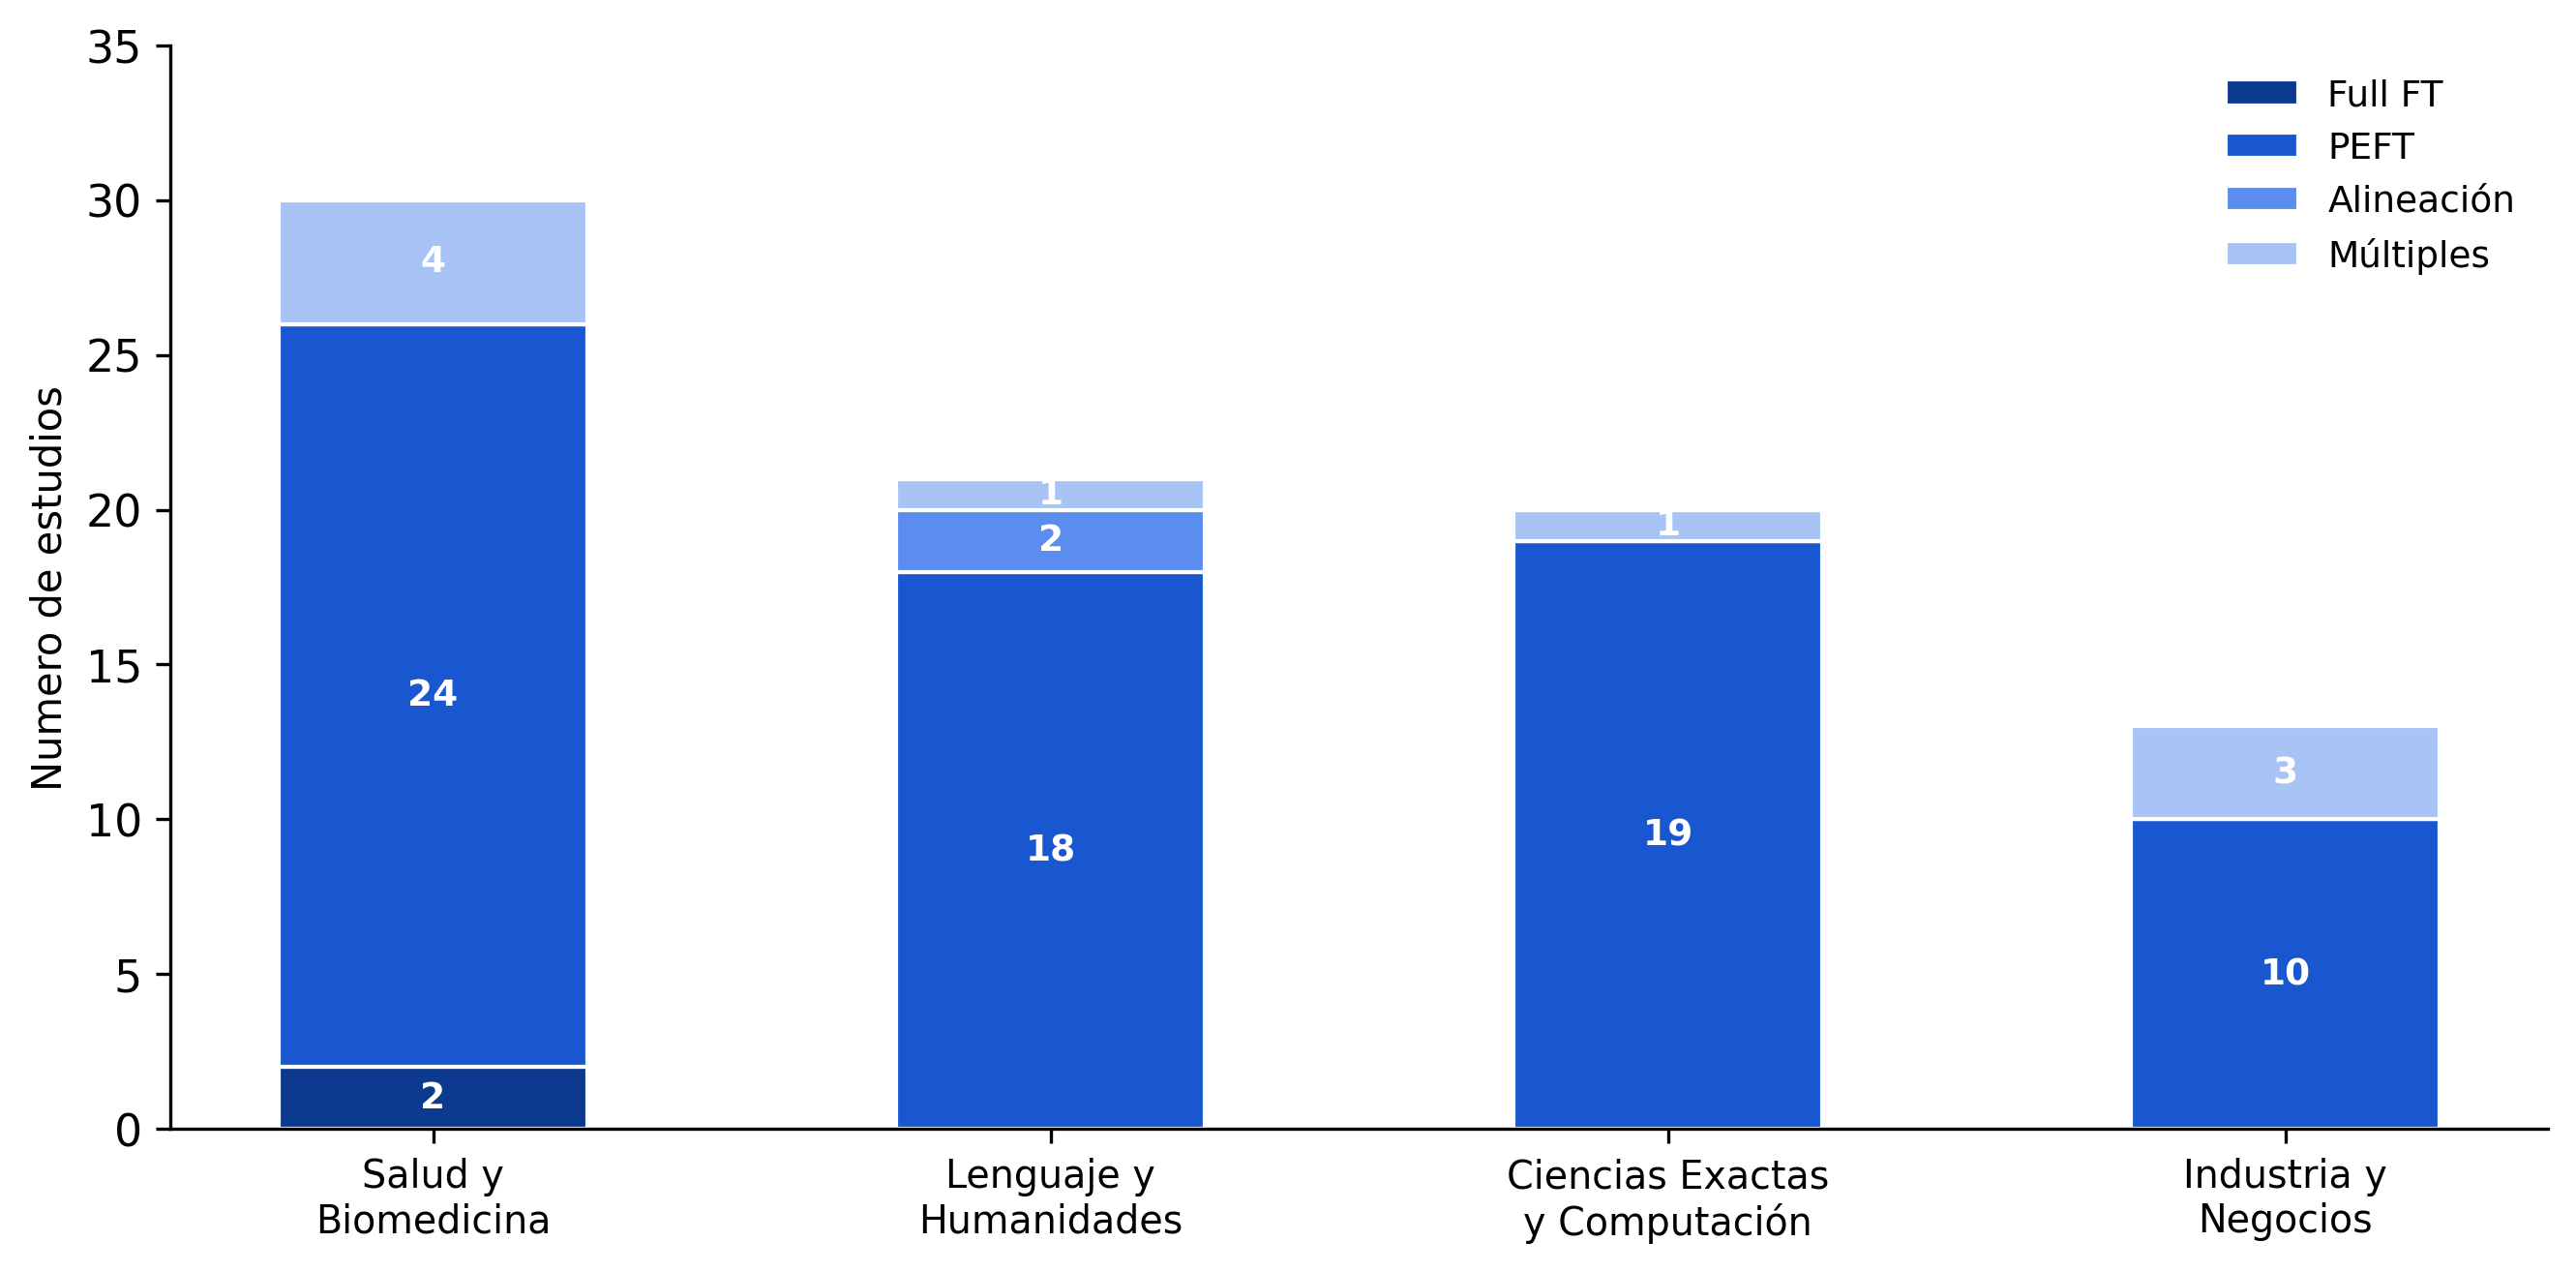
\includegraphics[width=0.9\linewidth]{Imagenes/fig4b_familias_por_dominio.png}
    \label{fig:familias}
    \begin{flushleft}
    \footnotesize
    \textit{Nota.} Las familias corresponden a las tres categorías definidas en el marco teórico: \textit{Full Fine-Tuning}, PEFT y Alineación. Un estudio puede contribuir a más de una familia si combina técnicas de distintas categorías.
    \end{flushleft}
\end{figure}

\begin{figure}[H]
    \centering
    \caption{Uso de técnicas específicas de \textit{fine-tuning} por dominio de aplicación (n = 84)}
    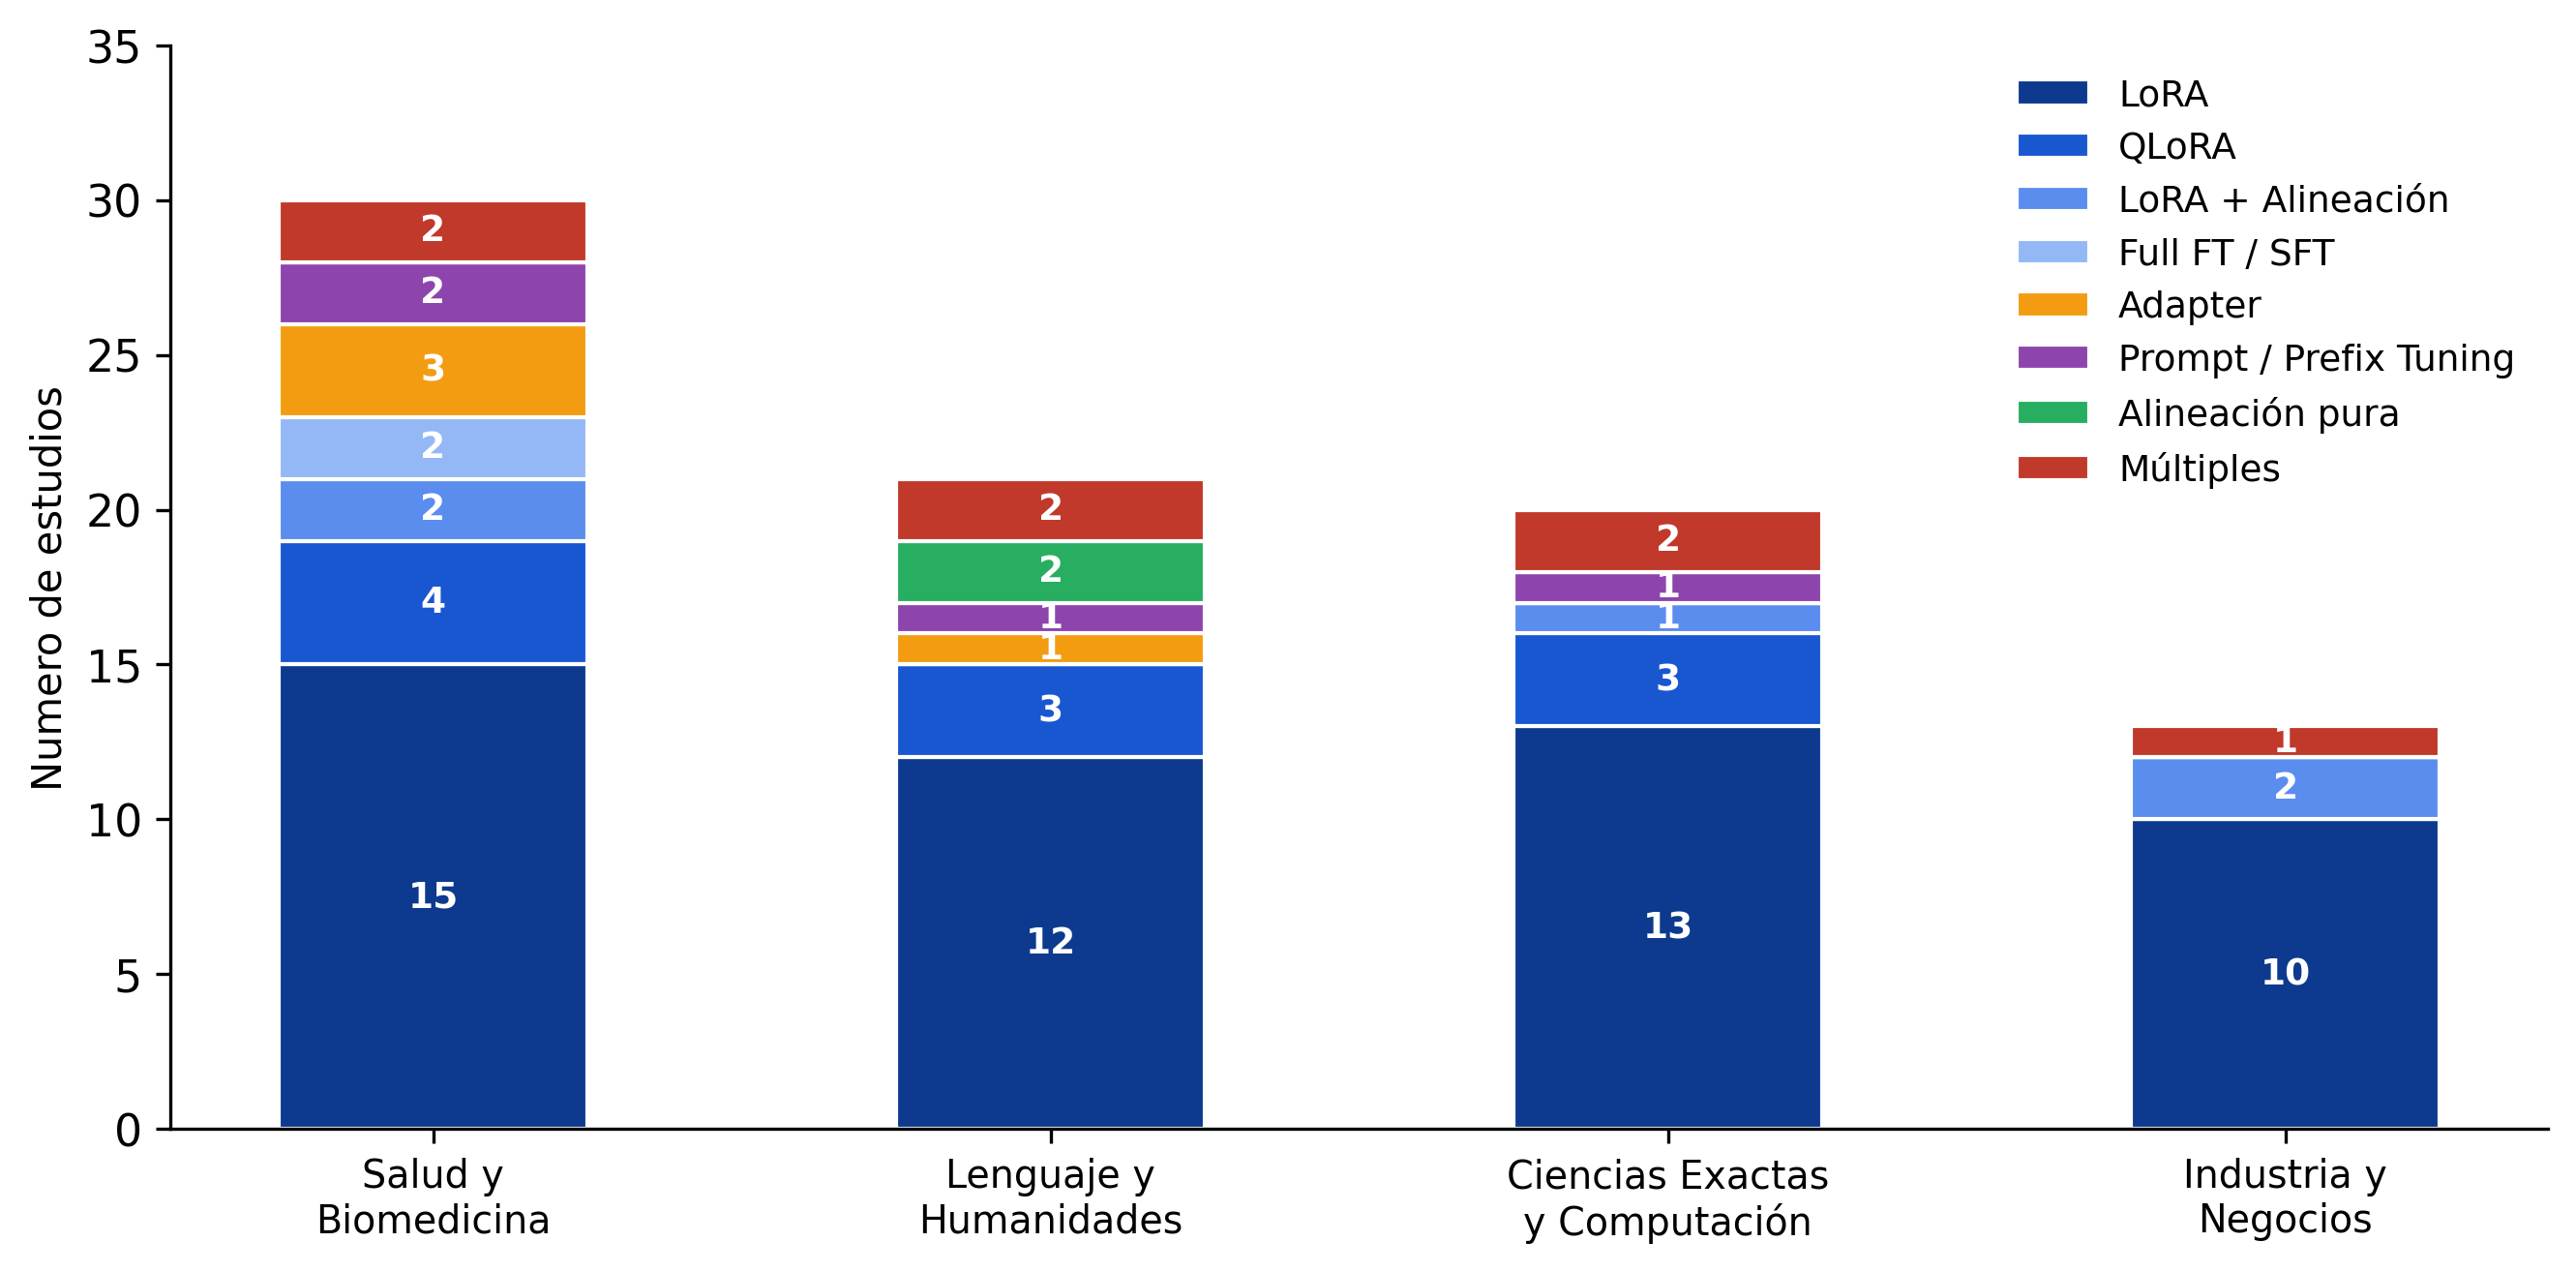
\includegraphics[width=0.9\linewidth]{Imagenes/fig4a_tecnicas_por_dominio.png}
    \label{fig:tecnicas}
    \begin{flushleft}
    \footnotesize
    \textit{Nota.} ``LoRA + Alineación'' agrupa estudios que combinan LoRA con RLHF, DPO u ORPO como mecanismo complementario. ``Alineación pura'' corresponde a estudios que aplican DPO u ORPO sin LoRA como técnica base. ``Múltiples'' agrupa estudios que combinan técnicas de distintas familias sin una técnica base dominante. Un estudio puede contabilizarse en más de una categoría si combina técnicas.
    \end{flushleft}
\end{figure}

La forma en que LoRA se combina con otras técnicas varía según el dominio. En Salud y Biomedicina aparece combinada con GRPO en reportes clínicos \parencite{kuo2025medical} y con otros mecanismos de adaptación complementaria. En Industria y Negocios predomina su combinación con RLHF para alineación \parencite{ren2025patent} y con RAG para recuperación de conocimiento especializado \parencite{xiong2025lora}. En contraste, Lenguaje y Humanidades y Ciencias Exactas y Computación presentan mayor proporción de estudios que usan LoRA de forma aislada, reflejando un carácter más experimental y comparativo \parencite{anghel2025courseeval, chen2025ft, xiang2024sumllama}.

%%%%%%%%%%%%%%%%%%%%%%%%%%%%%%%%%%%%%%%%
\subsection{Cobertura metodológica y reporte de métricas}

La proporción de estudios con pares de valores comparables (baseline y resultado explícitos) varía entre dominios. Salud y Biomedicina y Lenguaje y Humanidades presentan 9 estudios comparables cada uno (30,0\% y 42,9\% de sus respectivos dominios), Industria y Negocios 6 de 13 (46,2\%) y Ciencias Exactas y Computación 6 de 20 (30,0\%). La ausencia de valores comparables es más frecuente en dominios donde las contribuciones se centran en el diseño de sistemas o la evaluación cualitativa, como ocurre en Salud y en CyC, donde los jueces expertos o la ausencia de un único \textit{baseline} de referencia impiden el cálculo de mejora relativa.

Las métricas empleadas difieren según el dominio. F1 predomina en Salud y Biomedicina dado el énfasis en extracción de entidades y clasificación clínica \parencite{zhou2024adapter}. \textit{Accuracy} es la métrica más frecuente en Ciencias Exactas y Computación, donde los \textit{benchmarks} de razonamiento dominan \parencite{liu2025tasks}. En Lenguaje y Humanidades coexisten F1 \parencite{han2025ft}, \textit{accuracy} \parencite{kadyrbek2025dpo, shen2025ft} y métricas específicas de tarea como ROUGE-L en generación \parencite{chen2025ft}. En Industria y Negocios la heterogeneidad es máxima, con BLEU-4 \parencite{ren2025patent}, Macro-F1 \parencite{yang2025hierarchic} y ROUGE-L \parencite{song2025lora} distribuidos según la naturaleza de cada aplicación vertical.

%%%%%%%%%%%%%%%%%%%%%%%%%%%%%%%%%%%%%%%%
\subsection{Patrones transversales}

Tres patrones emergen de forma consistente a través de los cuatro dominios del corpus. La Figura~\ref{fig:mejoras} resume la dirección de los resultados reportados, mostrando que la gran mayoría de los estudios con métricas comparables reportan mejora positiva sobre sus \textit{baselines} de referencia.

\begin{figure}[H]
    \centering
    \caption{Dirección de la mejora respecto al \textit{baseline} por dominio (estudios con pares de valores comparables, n = 30)}
    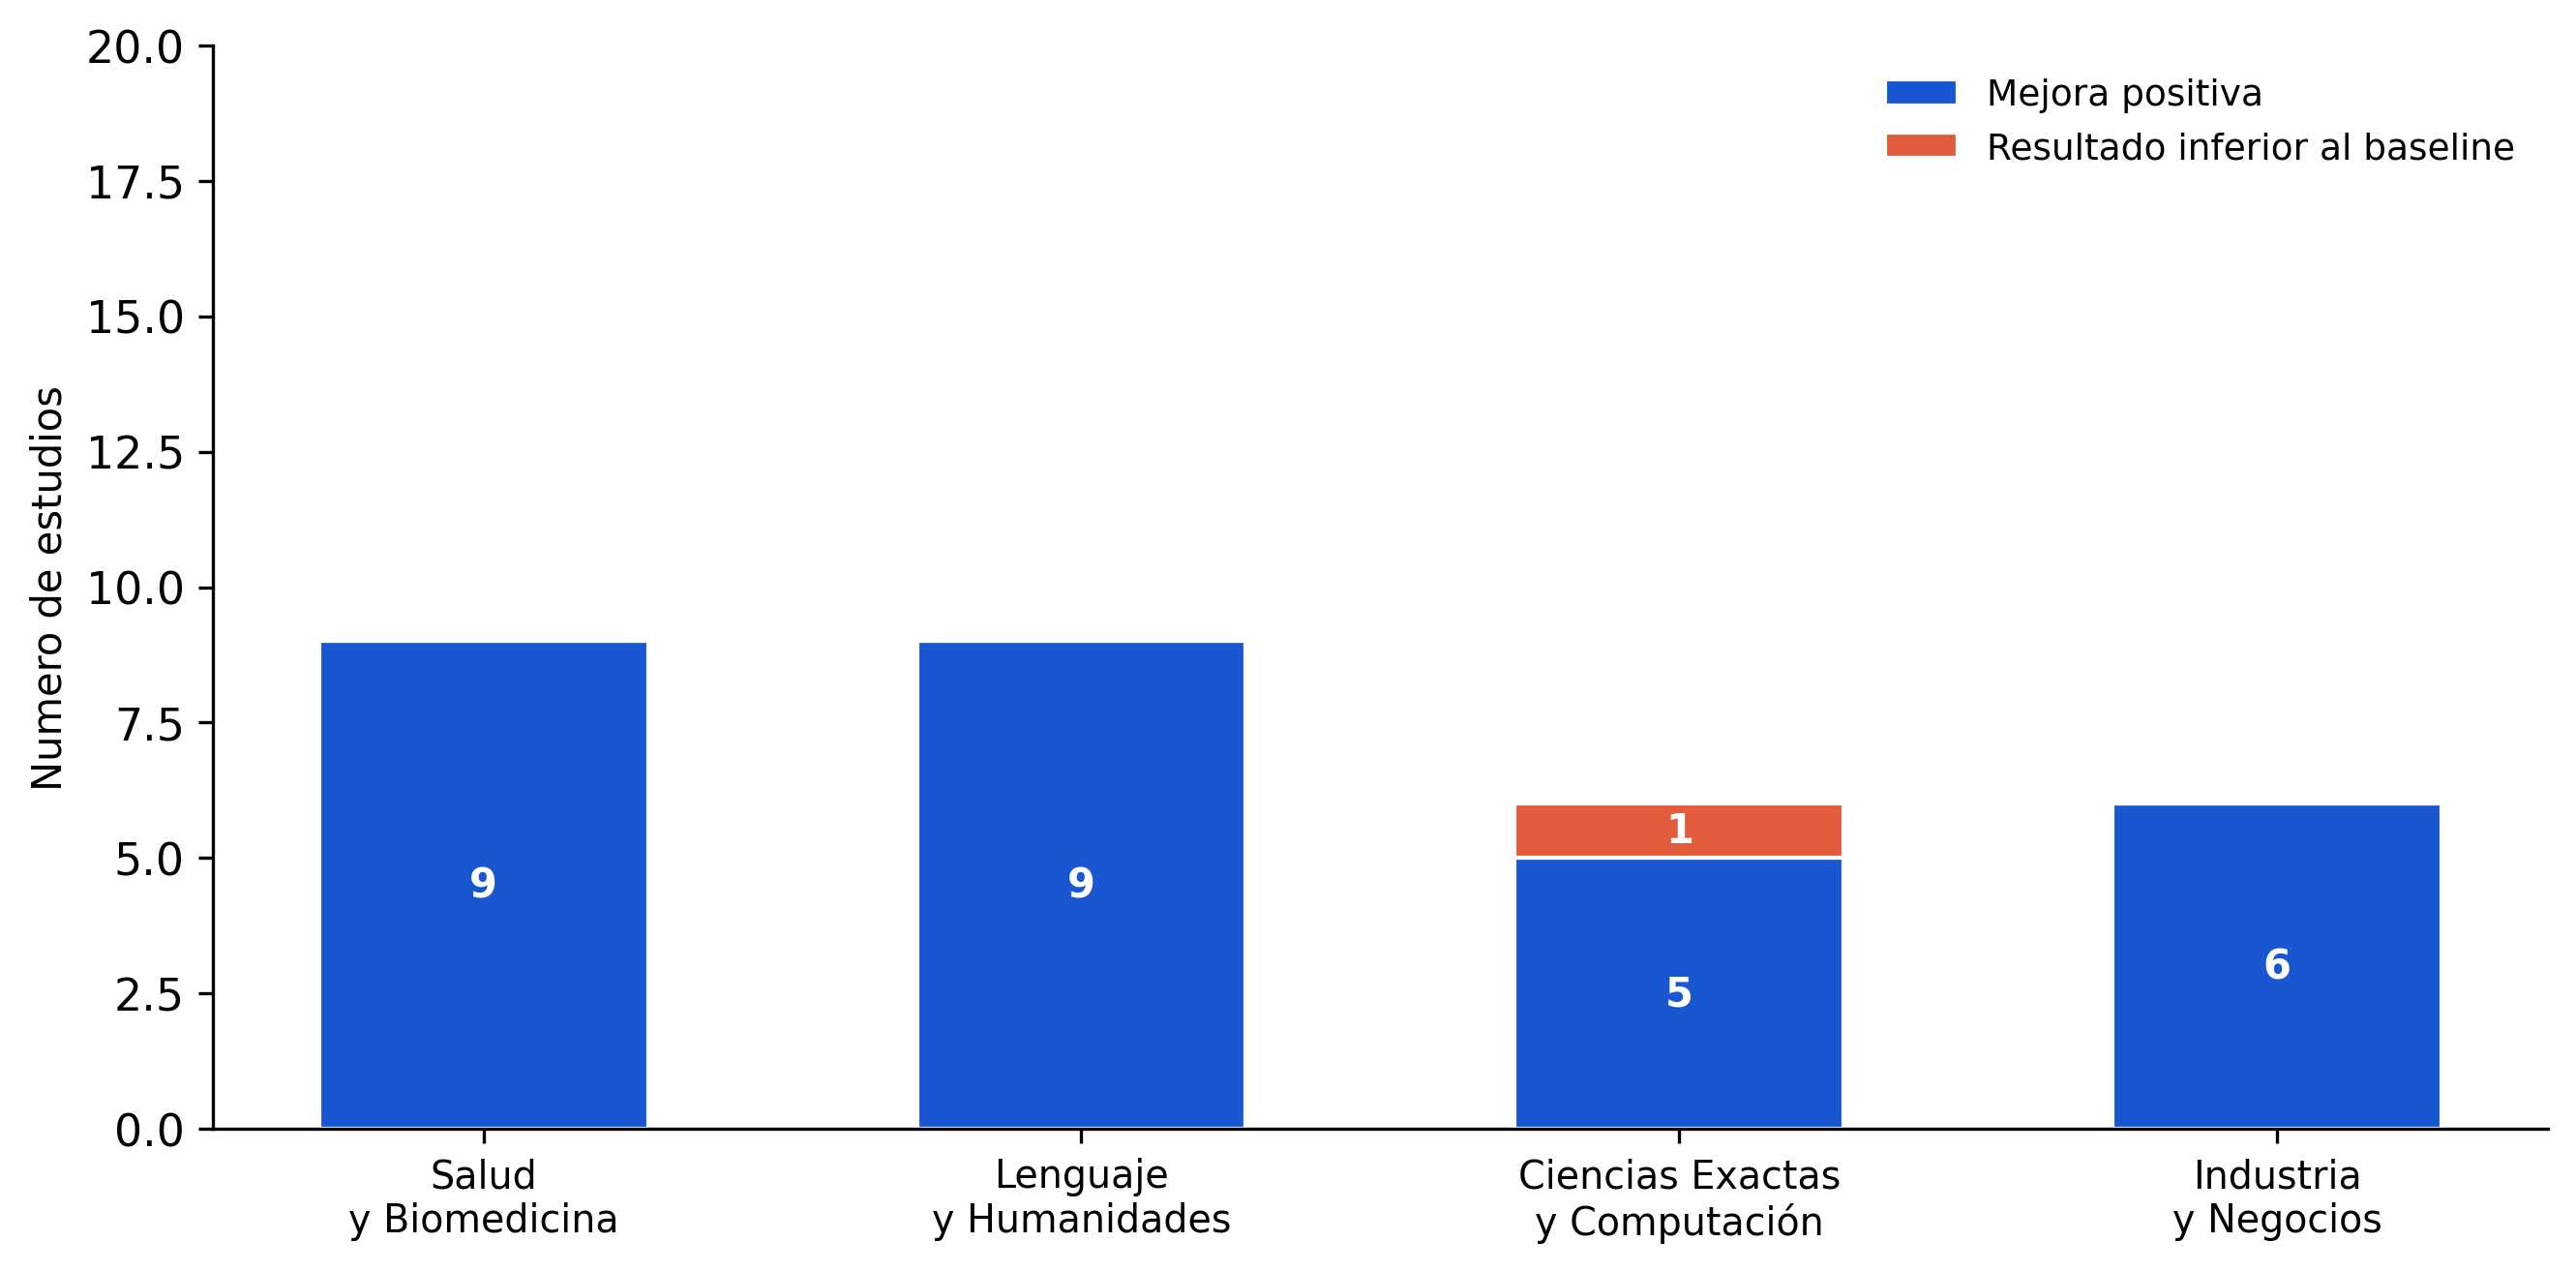
\includegraphics[width=0.9\linewidth]{Imagenes/fig5_direccion_mejoras.png}
    \label{fig:mejoras}
    \begin{flushleft}
    \footnotesize
    \textit{Nota.} Se incluyen únicamente los 30 estudios del corpus que declaran explícitamente un \textit{baseline} de referencia y reportan tanto el valor de referencia como el resultado obtenido tras el \textit{fine-tuning}, lo que permite calcular la dirección y magnitud del cambio. El único resultado negativo corresponde al dominio de Ciencias Exactas y Computación.
    \end{flushleft}
\end{figure}

El primer patrón es la dominancia transversal de LoRA como técnica de adaptación. LoRA o alguna de sus variantes está presente en 67 de los 84 estudios del corpus (79,8\%), con una frecuencia que se mantiene alta en todos los dominios sin excepción. Este patrón de adopción no depende de la tarea, el idioma ni el tamaño del modelo, lo que sugiere que LoRA ha consolidado su posición como técnica de referencia en la literatura de \textit{fine-tuning} de LLMs durante el período analizado.

El segundo patrón es la efectividad consistente del \textit{fine-tuning} sobre el modelo base sin adaptar. De los 30 estudios con pares de valores comparables, la dirección del cambio es positiva en 29 casos, con mejoras relativas que en varios estudios superan el 100\%. Este patrón se observa en dominios y tareas diversas: en diálogo geriátrico se reporta una mejora de ROUGE de 8,60\% a 34,96\% (+306,5\%) \parencite{xu2025cpel}, y en extracción de información militar una ganancia de Macro-F1 de 0,2140 a 0,7020 (+228,0\%) \parencite{yang2025hierarchic}. Es importante señalar que la heterogeneidad de métricas y \textit{datasets} entre estudios impide una agregación directa de valores absolutos; el patrón se establece a nivel de dirección de la mejora, no de magnitud promedio entre dominios.

El tercer patrón es la tendencia hacia arquitecturas compuestas en aplicaciones orientadas a producción. La familia PEFT, con LoRA como técnica predominante, no solo domina en frecuencia sino que en contextos aplicados tiende a combinarse con mecanismos complementarios: con RLHF para alineación de preferencias \parencite{ren2025patent}, con RAG para recuperación de conocimiento especializado \parencite{xiong2025lora} y con marcos de aprendizaje federado para privacidad distribuida \parencite{elbakary2025mira, liu2025federated}. Este patrón sugiere que la familia PEFT actúa como componente base sobre el que se construyen sistemas más complejos en aplicaciones de producción, especialmente en los dominios de Salud y Biomedicina e Industria y Negocios.
%%%%%%%%%%%%%%%%%%%%%%%%%%%%%%%%%%%%%%%%
\chapter{Conclusiones}
%%%%%%%%%%%%%%%%%%%%%%%%%%%%%%%%%%%%%%%%

La presente revisión sistemática analizó 84 estudios empíricos publicados entre 2020 y 2025 sobre técnicas de \textit{fine-tuning} para \textit{Large Language Models}, seleccionados mediante el protocolo PRISMA desde una búsqueda inicial de 140 registros en Scopus. Los hallazgos se organizan en correspondencia con los tres objetivos específicos planteados.

En relación con el primer objetivo, sistematizar la literatura mediante PRISMA extrayendo características técnicas, métricas y resultados por dominio, el corpus presenta una distribución heterogénea entre cuatro dominios de aplicación: Salud y Biomedicina (30 estudios), Lenguaje y Humanidades (21), Ciencias Exactas y Computación (20) e Industria y Negocios (13). LoRA y sus variantes, incluyendo QLoRA, emergen como la categoría dominante con presencia en el 79,8\% de los estudios (67 de 84). La calidad metodológica del corpus fue aceptable en conjunto, con un \textit{score} promedio de 2,61 sobre 3,0. La extracción de datos permitió documentar técnicas, modelos base, \textit{datasets}, métricas y resultados de forma estructurada y trazable para cada uno de los 84 estudios incluidos, cumpliendo los requisitos de reproducibilidad del protocolo PRISMA.

En relación con el segundo objetivo, analizar el rendimiento por dominio, los \textit{trade-offs} y los patrones de aplicabilidad, el análisis revela que el \textit{fine-tuning} paramétrico eficiente produce mejoras consistentes sobre el modelo base sin adaptar en todos los dominios evaluados, aunque con magnitudes variables según el contexto. Los estudios con métricas comparables muestran que las mejoras más consistentes se concentran en tareas de baja cobertura lingüística y dominios altamente especializados, donde el ajuste fino sobre datos del dominio produce ganancias sustanciales independientemente del tamaño del modelo. Los patrones de aplicabilidad difieren entre dominios: en Salud y Biomedicina predomina la preferencia por modelos abiertos motivada por restricciones de privacidad; en Lenguaje y Humanidades destaca la diversificación de variantes de LoRA orientadas a tareas específicas; en Ciencias Exactas y Computación LoRA se consolida como referencia establecida e integrada con aprendizaje federado; y en Industria y Negocios la configuración dominante combina LoRA con RLHF para tareas de generación de alto valor.

En relación con el tercer objetivo, sintetizar criterios de selección según contexto operativo, limitaciones y direcciones futuras, la evidencia acumulada permite formular tres criterios basados en evidencia empírica. Cuando existen restricciones de privacidad o se opera sobre datos sensibles, QLoRA sobre modelos abiertos es la configuración más respaldada por la literatura, con documentación explícita en estudios clínicos y biomédicos. Cuando el dominio de aplicación es altamente especializado o la lengua tiene baja cobertura en los datos de preentrenamiento, LoRA con \textit{datasets} específicos del dominio produce las mejoras más sustanciales independientemente del tamaño del modelo base. Cuando el objetivo es la calidad y alineación del texto generado en aplicaciones de producción, la combinación LoRA + RLHF es la configuración predominante en la literatura reciente, especialmente en dominios industriales y legales.

En respuesta a la pregunta de investigación, las técnicas de \textit{fine-tuning} para \textit{Large Language Models} desarrolladas entre 2020 y 2025 convergen hacia un modelo de adaptación paramétrica eficiente con LoRA como componente central, complementado con mecanismos adicionales según el contexto operativo. La selección de técnica no depende exclusivamente del rendimiento absoluto sino de factores contextuales como la privacidad de los datos, la disponibilidad de recursos lingüísticos del dominio y los requisitos de alineación de las respuestas generadas. Este patrón, consistente a través de dominios y tareas, sugiere que la comunidad investigadora ha convergido hacia un conjunto acotado de configuraciones efectivas durante el período analizado.

La presente revisión presenta cuatro limitaciones principales que deben considerarse al interpretar sus hallazgos. La primera es la restricción a una única base de datos: la búsqueda se realizó exclusivamente en Scopus, lo que puede haber excluido estudios relevantes indexados únicamente en IEEE Xplore, ACM Digital Library o disponibles como preprints en arXiv. La segunda es la heterogeneidad de \textit{baselines}: los estudios incluidos emplean referencias de comparación de naturaleza diversa, lo que impide una síntesis cuantitativa unificada y limita la comparación directa de magnitudes de mejora entre estudios y dominios. La tercera es la ausencia de \textit{baseline} explícito en el 64,3\% de los estudios incluidos (54 de 84), lo que concentra las comparaciones en el subconjunto con reporte completo. La cuarta es el sesgo de acceso abierto: el filtro aplicado para garantizar la reproducibilidad del proceso de extracción puede haber introducido un sesgo de selección hacia ciertos tipos de publicaciones o dominios con mayor tradición de publicación abierta.

Los hallazgos de esta revisión sugieren tres direcciones prioritarias para la investigación futura. La primera es la estandarización de protocolos de evaluación y reporte: la heterogeneidad de métricas, \textit{baselines} y configuraciones experimentales documentada en este corpus dificulta la acumulación de evidencia comparativa, y el desarrollo de estándares análogos a los existentes en otras áreas de \textit{machine learning} permitiría síntesis cuantitativas más robustas. La segunda es la investigación en escenarios de recursos limitados: los hallazgos más consistentes del corpus corresponden a adaptaciones en lenguas de baja cobertura y dominios con datos escasos, y la investigación futura debería profundizar en el tamaño mínimo de \textit{dataset} necesario para obtener mejoras significativas y en la sensibilidad a la calidad de los datos de entrenamiento. La tercera es la evaluación comparativa de técnicas de alineación: RLHF y DPO aparecen en el corpus principalmente en dominios aplicados pero con escasa evidencia cuantitativa comparativa entre ellas, y estudios que las comparen sistemáticamente con métricas y \textit{baselines} compartidos contribuirían a orientar la selección de técnica en aplicaciones de producción.

%%%%%%%%%%%%%%%%%%%%%%%%%%%%%%%%%%%%%%%%
\nocite{*}
\printbibliography
%%%%%%%%%%%%%%%%%%%%%%%%%%%%%%%%%%%%%%%%

%%%%%%%%%%%%%%%%%%%%%%%%%%%%%%%%%%%%%%%%
\chapter{Apéndices}
%%%%%%%%%%%%%%%%%%%%%%%%%%%%%%%%%%%%%%%%

%%%%%%%%%%%%%%%%%%%%%%%%%%%%%%%%%%%%%%%%
\section*{Apéndice A: Corpus completo de estudios incluidos}
\addcontentsline{toc}{section}{Apéndice A: Corpus completo de estudios incluidos}

Las tablas siguientes presentan los 84 estudios incluidos en la revisión sistemática, organizados por dominio de aplicación. Para cada estudio se reporta la técnica principal de \textit{fine-tuning}, la tarea evaluada, la métrica principal de evaluación declarada por los autores, el valor del \textit{baseline} de referencia y el resultado reportado, junto con el cambio porcentual relativo ($\Delta$\%) calculado sobre la misma métrica. Los valores negativos de $\Delta$\% indican que la técnica evaluada no superó al \textit{baseline}.

%%%%%%%%%%%%%%%%%%%%%%%%%%%%%%%%%%%%%%%%
\subsection*{A.1 \quad Salud y Biomedicina \texorpdfstring{(n = 30)}{(n = 30)}}
\addcontentsline{toc}{subsection}{A.1 Salud y Biomedicina}

\begin{longtable}{p{3.5cm} p{1.7cm} p{3.0cm} p{1.8cm} p{1.3cm} p{1.3cm} p{0.9cm}}
\caption{Corpus completo -- Salud y Biomedicina (n = 30).} \label{tab:apx_salud} \\
\toprule
\scriptsize\textbf{Referencia} & \scriptsize\textbf{Técnica} & \scriptsize\textbf{Tarea} & \scriptsize\textbf{Métrica principal} & \scriptsize\textbf{Baseline} & \scriptsize\textbf{Resultado} & \scriptsize\textbf{$\Delta$\%} \\
\midrule
\endfirsthead
\multicolumn{7}{l}{\scriptsize\textit{Tabla \ref{tab:apx_salud} -- continuación}} \\[2pt]
\toprule
\scriptsize\textbf{Referencia} & \scriptsize\textbf{Técnica} & \scriptsize\textbf{Tarea} & \scriptsize\textbf{Métrica principal} & \scriptsize\textbf{Baseline} & \scriptsize\textbf{Resultado} & \scriptsize\textbf{$\Delta$\%} \\
\midrule
\endhead
\midrule
\multicolumn{7}{r}{\scriptsize\textit{Continúa en la página siguiente}} \\
\endfoot
\bottomrule
\endlastfoot
\multicolumn{7}{l}{\scriptsize\textbf{\textit{Full Fine-Tuning}}} \\[2pt]
\scriptsize\autocite{sousa2025medical} & \scriptsize Full FT & \scriptsize Desidentificación & \scriptsize --- & \scriptsize --- & \scriptsize --- & \scriptsize --- \\
\scriptsize\autocite{xu2024mentalllm} & \scriptsize IT & \scriptsize Clasif. salud mental & \scriptsize --- & \scriptsize --- & \scriptsize --- & \scriptsize --- \\
\multicolumn{7}{l}{\scriptsize\textbf{\textit{PEFT}}} \\[2pt]
\scriptsize\autocite{nowak2025privacy} & \scriptsize\textit{LoRA} & \scriptsize Extracción clínica & \scriptsize --- & \scriptsize --- & \scriptsize --- & \scriptsize --- \\
\scriptsize\autocite{zhang2025dialogue} & \scriptsize\textit{Adapter} & \scriptsize Diálogo con conocimiento & \scriptsize --- & \scriptsize --- & \scriptsize --- & \scriptsize --- \\
\scriptsize\autocite{zhou2024adapter} & \scriptsize\textit{Adapter} & \scriptsize NER médico (chino) & \scriptsize --- & \scriptsize --- & \scriptsize --- & \scriptsize --- \\
\scriptsize\autocite{zhao2025daft} & \scriptsize\textit{DAFT} & \scriptsize Desinformación en salud & \scriptsize Accuracy & \scriptsize 76,95\% & \scriptsize 84,77\% & \scriptsize +10,2\% \\
\scriptsize\autocite{adhikary2025medical} & \scriptsize\textit{LoRA} & \scriptsize Q\&A salud menstrual & \scriptsize --- & \scriptsize --- & \scriptsize --- & \scriptsize --- \\
\scriptsize\autocite{bayram2025medical} & \scriptsize\textit{LoRA} & \scriptsize Q\&A médico (turco) & \scriptsize Similitud & \scriptsize 0,4627 & \scriptsize 0,5151 & \scriptsize +11,3\% \\
\scriptsize\autocite{elmitwalli2024ft} & \scriptsize\textit{LoRA} & \scriptsize Análisis de sentimiento & \scriptsize Accuracy & \scriptsize 0,65 & \scriptsize 0,94 & \scriptsize +44,6\% \\
\scriptsize\autocite{khader2025ft} & \scriptsize\textit{LoRA} & \scriptsize Q\&A médico (árabe) & \scriptsize --- & \scriptsize --- & \scriptsize --- & \scriptsize --- \\
\scriptsize\autocite{li2025tcmds} & \scriptsize\textit{LoRA} & \scriptsize Recom. fórmulas TCM & \scriptsize Precision & \scriptsize 0,3848 & \scriptsize 0,9924 & \scriptsize +157,9\% \\
\scriptsize\autocite{qi2025transformi} & \scriptsize\textit{LoRA} & \scriptsize Diálogo terapia ABA & \scriptsize --- & \scriptsize --- & \scriptsize --- & \scriptsize --- \\
\scriptsize\autocite{richterpechanski2025medication} & \scriptsize\textit{LoRA} & \scriptsize Extracción medicamentos & \scriptsize --- & \scriptsize --- & \scriptsize --- & \scriptsize --- \\
\scriptsize\autocite{tong2025xuanhugpt} & \scriptsize\textit{LoRA} & \scriptsize Q\&A medicina TCM & \scriptsize --- & \scriptsize --- & \scriptsize --- & \scriptsize --- \\
\scriptsize\autocite{tran2024bioinstruct} & \scriptsize\textit{LoRA} & \scriptsize Q\&A biomédico & \scriptsize --- & \scriptsize --- & \scriptsize --- & \scriptsize --- \\
\scriptsize\autocite{vithanage2025medical} & \scriptsize\textit{LoRA} & \scriptsize NER clínico & \scriptsize --- & \scriptsize --- & \scriptsize --- & \scriptsize --- \\
\scriptsize\autocite{xu2025cpel} & \scriptsize\textit{LoRA} & \scriptsize Diálogo geriátrico & \scriptsize ROUGE & \scriptsize 8,60\% & \scriptsize 34,96\% & \scriptsize +306,5\% \\
\scriptsize\autocite{yang2024tcmgpt} & \scriptsize\textit{LoRA} & \scriptsize Medicina tradicional & \scriptsize Accuracy & \scriptsize 0,247 & \scriptsize 0,290 & \scriptsize +17,4\% \\
\scriptsize\autocite{bao2025ecbti} & \scriptsize\textit{LoRA} & \scriptsize Diálogo terapéutico & \scriptsize --- & \scriptsize --- & \scriptsize --- & \scriptsize --- \\
\scriptsize\autocite{liu2024cpmi} & \scriptsize P-Tuning v2 & \scriptsize Prescripción TCM & \scriptsize --- & \scriptsize --- & \scriptsize --- & \scriptsize --- \\
\scriptsize\autocite{yang2025ceprompt} & \scriptsize\textit{Prompt Tuning} & \scriptsize Q\&A médico (KG) & \scriptsize --- & \scriptsize --- & \scriptsize --- & \scriptsize --- \\
\scriptsize\autocite{bui2025ft} & \scriptsize\textit{LoRA} & \scriptsize Q\&A médico (vietnamita) & \scriptsize --- & \scriptsize --- & \scriptsize --- & \scriptsize --- \\
\scriptsize\autocite{chao2025evaluating} & \scriptsize\textit{QLoRA} & \scriptsize Resumen clínico & \scriptsize --- & \scriptsize --- & \scriptsize --- & \scriptsize --- \\
\scriptsize\autocite{dietrich2025ner} & \scriptsize\textit{QLoRA} & \scriptsize NER farmacovigilancia & \scriptsize --- & \scriptsize --- & \scriptsize --- & \scriptsize --- \\
\scriptsize\autocite{dormus2025harnessing} & \scriptsize\textit{QLoRA} & \scriptsize Desidentificación & \scriptsize --- & \scriptsize --- & \scriptsize --- & \scriptsize --- \\
\scriptsize\autocite{hou2024ft} & \scriptsize\textit{QLoRA} & \scriptsize Gen. cartas médicas & \scriptsize ROUGE-1 & \scriptsize 0,161 & \scriptsize 0,352 & \scriptsize +118,6\% \\
\multicolumn{7}{l}{\scriptsize\textbf{\textit{Múltiples}}} \\[2pt]
\scriptsize\autocite{zhu2025fullft} & \scriptsize Full FT (GaLore) & \scriptsize Prev. lesiones deportivas & \scriptsize BLEU-4 & \scriptsize 29,415 & \scriptsize 29,589 & \scriptsize +0,6\% \\
\scriptsize\autocite{rullo2025cardio} & \scriptsize\textit{LoRA}+GRPO & \scriptsize Educación cardiovascular (HIV) & \scriptsize Human Eval. Accuracy & \scriptsize 4,16 & \scriptsize 5,0 & \scriptsize +20,2\% \\
\scriptsize\autocite{kuo2025medical} & \scriptsize\textit{LoRA}+GRPO & \scriptsize Reportes clínicos & \scriptsize --- & \scriptsize --- & \scriptsize --- & \scriptsize --- \\
\scriptsize\autocite{savage2025dpo} & \scriptsize SFT+DPO & \scriptsize Razonamiento clínico & \scriptsize --- & \scriptsize --- & \scriptsize --- & \scriptsize --- \\
\end{longtable}

\begin{flushleft}
\scriptsize
\textit{Nota.} IT = \textit{Instruction Tuning}; Full FT = \textit{Full Fine-Tuning}; SFT = \textit{Supervised Fine-Tuning}; DPO = \textit{Direct Preference Optimization}; GRPO = \textit{Group Relative Policy Optimization}; DAFT = \textit{Domain-Augmented Fine-Tuning}; GaLore = \textit{Gradient Low-Rank Projection}; TCM = \textit{Traditional Chinese Medicine} (medicina tradicional china); KG = \textit{Knowledge Graph} (grafo de conocimiento); NER = \textit{Named Entity Recognition} (reconocimiento de entidades nombradas); ABA = \textit{Applied Behavior Analysis} (análisis conductual aplicado); Human Eval.\ Accuracy = exactitud evaluada por jueces humanos en escala numérica definida por cada estudio (escala 1-5 en \autocite{rullo2025cardio}). Los guiones (---) en las columnas Baseline, Resultado y $\Delta$\% indican que el estudio no reporta un par de comparación homogéneo que permita calcular una mejora relativa, ya sea porque evalúa múltiples técnicas o modelos sin un \textit{baseline} único de referencia, o porque los resultados no son directamente comparables entre sí.
\end{flushleft}

%%%%%%%%%%%%%%%%%%%%%%%%%%%%%%%%%%%%%%%%
\subsection*{A.2 \quad Lenguaje y Humanidades \texorpdfstring{(n = 21)}{(n = 21)}}
\addcontentsline{toc}{subsection}{A.2 Lenguaje y Humanidades}

\begin{longtable}{p{3.5cm} p{1.7cm} p{3.0cm} p{1.8cm} p{1.3cm} p{1.3cm} p{0.9cm}}
\caption{Corpus completo -- Lenguaje y Humanidades (n = 21).} \label{tab:apx_lh} \\
\toprule
\scriptsize\textbf{Referencia} & \scriptsize\textbf{Técnica} & \scriptsize\textbf{Tarea} & \scriptsize\textbf{Métrica principal} & \scriptsize\textbf{Baseline} & \scriptsize\textbf{Resultado} & \scriptsize\textbf{$\Delta$\%} \\
\midrule
\endfirsthead
\multicolumn{7}{l}{\scriptsize\textit{Tabla \ref{tab:apx_lh} -- continuación}} \\[2pt]
\toprule
\scriptsize\textbf{Referencia} & \scriptsize\textbf{Técnica} & \scriptsize\textbf{Tarea} & \scriptsize\textbf{Métrica principal} & \scriptsize\textbf{Baseline} & \scriptsize\textbf{Resultado} & \scriptsize\textbf{$\Delta$\%} \\
\midrule
\endhead
\midrule
\multicolumn{7}{r}{\scriptsize\textit{Continúa en la página siguiente}} \\
\endfoot
\bottomrule
\endlastfoot
\multicolumn{7}{l}{\scriptsize\textbf{\textit{PEFT}}} \\[2pt]
\scriptsize\autocite{chen2025adaptforever} & \scriptsize\textit{Adapter} & \scriptsize Clasificación GLUE & \scriptsize Promedio & \scriptsize 86,4 & \scriptsize 89,0 & \scriptsize +3,0\% \\
\scriptsize\autocite{anghel2025courseeval} & \scriptsize\textit{LoRA} & \scriptsize Evaluación educativa & \scriptsize Human Eval. Accuracy & \scriptsize 7,94 & \scriptsize 8,21 & \scriptsize +3,4\% \\
\scriptsize\autocite{chen2025ft} & \scriptsize\textit{LoRA} & \scriptsize Q\&A patrimonio cultural & \scriptsize ROUGE-L & \scriptsize 22,39\% & \scriptsize 47,85\% & \scriptsize +113,7\% \\
\scriptsize\autocite{han2025ft} & \scriptsize\textit{LoRA} & \scriptsize Detección de duplicados & \scriptsize F1 & \scriptsize 82,02\% & \scriptsize 84,90\% & \scriptsize +3,5\% \\
\scriptsize\autocite{harris2025benchmark} & \scriptsize\textit{LoRA} & \scriptsize Fake news (urdu) & \scriptsize --- & \scriptsize --- & \scriptsize --- & \scriptsize --- \\
\scriptsize\autocite{kiziltepe2025ft} & \scriptsize\textit{LoRA} & \scriptsize Sentimiento (turco) & \scriptsize --- & \scriptsize --- & \scriptsize --- & \scriptsize --- \\
\scriptsize\autocite{li2025keft} & \scriptsize\textit{LoRA} & \scriptsize Q\&A general & \scriptsize --- & \scriptsize --- & \scriptsize --- & \scriptsize --- \\
\scriptsize\autocite{meng2025triplanet} & \scriptsize\textit{LoRA} & \scriptsize Detección de plagio & \scriptsize --- & \scriptsize --- & \scriptsize --- & \scriptsize --- \\
\scriptsize\autocite{rathore2025ft} & \scriptsize\textit{LoRA} & \scriptsize Discurso de odio & \scriptsize --- & \scriptsize --- & \scriptsize --- & \scriptsize --- \\
\scriptsize\autocite{wang2025lora} & \scriptsize DS-LoRA & \scriptsize Lenguaje ofensivo & \scriptsize Macro-F1 & \scriptsize 80,1 & \scriptsize 81,3 & \scriptsize +1,5\% \\
\scriptsize\autocite{ye2025loraadv} & \scriptsize\textit{LoRA} & \scriptsize Texto ofensivo & \scriptsize --- & \scriptsize --- & \scriptsize --- & \scriptsize --- \\
\scriptsize\autocite{zain2025ruold} & \scriptsize\textit{LoRA} & \scriptsize Lenguaje ofensivo (urdu) & \scriptsize --- & \scriptsize --- & \scriptsize --- & \scriptsize --- \\
\scriptsize\autocite{jia2025agnostic} & \scriptsize Multi-PEFT & \scriptsize Clasif. multi-tarea & \scriptsize Macro-F1 & \scriptsize 0,8712 & \scriptsize 0,8736 & \scriptsize +0,3\% \\
\scriptsize\autocite{cheng2025prompt} & \scriptsize\textit{Prompt Tuning} & \scriptsize KGQA multidominio & \scriptsize --- & \scriptsize --- & \scriptsize --- & \scriptsize --- \\
\scriptsize\autocite{huang2024quant} & \scriptsize\textit{QLoRA} & \scriptsize Cuantización LLMs & \scriptsize --- & \scriptsize --- & \scriptsize --- & \scriptsize --- \\
\scriptsize\autocite{khoboko2025ft} & \scriptsize\textit{QLoRA} & \scriptsize Traducción inglés-zulú & \scriptsize F1 & \scriptsize 10,52 & \scriptsize 42 & \scriptsize +299,2\% \\
\scriptsize\autocite{paiola2025bode} & \scriptsize\textit{QLoRA} & \scriptsize Benchmarks port. bras. & \scriptsize --- & \scriptsize --- & \scriptsize --- & \scriptsize --- \\
\scriptsize\autocite{sindhujan2025translation} & \scriptsize\textit{LoRA} & \scriptsize Quality Estimation (QE) sin referencia & \scriptsize --- & \scriptsize --- & \scriptsize --- & \scriptsize --- \\
\multicolumn{7}{l}{\scriptsize\textbf{\textit{Alineación}}} \\[2pt]
\scriptsize\autocite{kadyrbek2025dpo} & \scriptsize DPO & \scriptsize Q\&A en kazajo & \scriptsize Accuracy & \scriptsize 56,5\% & \scriptsize 62,7\% & \scriptsize +11,0\% \\
\scriptsize\autocite{shen2025ft} & \scriptsize ORPO & \scriptsize Análisis de sentimiento & \scriptsize Accuracy & \scriptsize 75,33\% & \scriptsize 86,67\% & \scriptsize +15,1\% \\
\multicolumn{7}{l}{\scriptsize\textbf{\textit{Múltiples}}} \\[2pt]
\scriptsize\autocite{sun2025dialoguemllm} & \scriptsize\textit{LoRA}+IT & \scriptsize Reconoc. de emociones & \scriptsize --- & \scriptsize --- & \scriptsize --- & \scriptsize --- \\
\end{longtable}

\begin{flushleft}
\scriptsize
\textit{Nota.} IT = \textit{Instruction Tuning}; DPO = \textit{Direct Preference Optimization}; ORPO = \textit{Odds Ratio Preference Optimization}; DS-LoRA = variante de \textit{LoRA} propuesta por los autores; Multi-PEFT = combinación de múltiples métodos \textit{PEFT}; GLUE = \textit{General Language Understanding Evaluation}; KGQA = \textit{Knowledge Graph Question Answering}; QE = \textit{Quality Estimation} (estimación de calidad de traducción sin referencia); Human Eval.\ Accuracy = exactitud evaluada por jueces humanos en escala numérica definida por cada estudio (escala 0-10 en \autocite{anghel2025courseeval}). Los guiones (---) en las columnas Baseline, Resultado y $\Delta$\% indican que el estudio no reporta un par de comparación homogéneo que permita calcular una mejora relativa, ya sea porque evalúa múltiples técnicas o modelos sin un \textit{baseline} único de referencia, o porque los resultados no son directamente comparables entre sí.
\end{flushleft}

%%%%%%%%%%%%%%%%%%%%%%%%%%%%%%%%%%%%%%%%
\subsection*{A.3 \quad Ciencias Exactas y Computación \texorpdfstring{(n = 20)}{(n = 20)}}
\addcontentsline{toc}{subsection}{A.3 Ciencias Exactas y Computación}

\begin{longtable}{p{3.5cm} p{1.7cm} p{3.0cm} p{1.8cm} p{1.3cm} p{1.3cm} p{0.9cm}}
\caption{Corpus completo -- Ciencias Exactas y Computación (n = 20).} \label{tab:apx_cec} \\
\toprule
\scriptsize\textbf{Referencia} & \scriptsize\textbf{Técnica} & \scriptsize\textbf{Tarea} & \scriptsize\textbf{Métrica principal} & \scriptsize\textbf{Baseline} & \scriptsize\textbf{Resultado} & \scriptsize\textbf{$\Delta$\%} \\
\midrule
\endfirsthead
\multicolumn{7}{l}{\scriptsize\textit{Tabla \ref{tab:apx_cec} -- continuación}} \\[2pt]
\toprule
\scriptsize\textbf{Referencia} & \scriptsize\textbf{Técnica} & \scriptsize\textbf{Tarea} & \scriptsize\textbf{Métrica principal} & \scriptsize\textbf{Baseline} & \scriptsize\textbf{Resultado} & \scriptsize\textbf{$\Delta$\%} \\
\midrule
\endhead
\midrule
\multicolumn{7}{r}{\scriptsize\textit{Continúa en la página siguiente}} \\
\endfoot
\bottomrule
\endlastfoot
\multicolumn{7}{l}{\scriptsize\textbf{\textit{PEFT}}} \\[2pt]
\scriptsize\autocite{liu2025federated} & \scriptsize DP-LoRA & \scriptsize PEFT federado privado & \scriptsize --- & \scriptsize --- & \scriptsize --- & \scriptsize --- \\
\scriptsize\autocite{ao2025lora} & \scriptsize SPLoRA & \scriptsize Seguridad en \textit{fine-tuning} & \scriptsize --- & \scriptsize --- & \scriptsize --- & \scriptsize --- \\
\scriptsize\autocite{chen2025glr} & \scriptsize\textit{LoRA} & \scriptsize Razon. sobre grafos & \scriptsize --- & \scriptsize --- & \scriptsize --- & \scriptsize --- \\
\scriptsize\autocite{elbakary2025mira} & \scriptsize\textit{LoRA} & \scriptsize Aprendizaje federado & \scriptsize --- & \scriptsize --- & \scriptsize --- & \scriptsize --- \\
\scriptsize\autocite{gogineni2025ft} & \scriptsize\textit{LoRA} & \scriptsize Optimización de eficiencia en \textit{fine-tuning} (GPU) & \scriptsize --- & \scriptsize --- & \scriptsize --- & \scriptsize --- \\
\scriptsize\autocite{iftikhar2025peft} & \scriptsize\textit{LoRA} & \scriptsize Sentimiento (FL) & \scriptsize Accuracy & \scriptsize 71,2\% & \scriptsize 73,8\% & \scriptsize +3,7\% \\
\scriptsize\autocite{li2025federated} & \scriptsize\textit{LoRA} & \scriptsize PEFT federado & \scriptsize Avg. Acc. & \scriptsize 76,6\% & \scriptsize 75,4\% & \scriptsize -1,6\% \\
\scriptsize\autocite{liu2025mpctf} & \scriptsize\textit{LoRA} & \scriptsize Entren. multi-parte & \scriptsize Accuracy & \scriptsize 14,25 & \scriptsize 65,43 & \scriptsize +359,2\% \\
\scriptsize\autocite{seo2025lora} & \scriptsize\textit{LoRA} & \scriptsize Reducción de overhead en SFT con packing & \scriptsize --- & \scriptsize --- & \scriptsize --- & \scriptsize --- \\
\scriptsize\autocite{wang2025ft} & \scriptsize\textit{LoRA} & \scriptsize Razon. sentido común & \scriptsize --- & \scriptsize --- & \scriptsize --- & \scriptsize --- \\
\scriptsize\autocite{wu2024federated} & \scriptsize\textit{LoRA} & \scriptsize Clasif. datos sensibles & \scriptsize --- & \scriptsize --- & \scriptsize --- & \scriptsize --- \\
\scriptsize\autocite{xiang2024sumllama} & \scriptsize\textit{LoRA} & \scriptsize Resumen bug reports & \scriptsize ROUGE-L & \scriptsize 39,69 & \scriptsize 41,01 & \scriptsize +3,3\% \\
\scriptsize\autocite{prottasha2024peft} & \scriptsize Múltiples & \scriptsize Clasificación de texto y NLU multi-tarea & \scriptsize --- & \scriptsize --- & \scriptsize --- & \scriptsize --- \\
\scriptsize\autocite{zou2025peft} & \scriptsize Múltiples & \scriptsize Ing. de software & \scriptsize --- & \scriptsize --- & \scriptsize --- & \scriptsize --- \\
\scriptsize\autocite{jung2025prefix} & \scriptsize\textit{Prefix Tuning} & \scriptsize Clasificación GLUE & \scriptsize --- & \scriptsize --- & \scriptsize --- & \scriptsize --- \\
\scriptsize\autocite{liu2025tasks} & \scriptsize\textit{Prompt Tuning}+\textit{LoRA} & \scriptsize Razon. SuperGLUE & \scriptsize --- & \scriptsize --- & \scriptsize --- & \scriptsize --- \\
\scriptsize\autocite{choi2025agentreport} & \scriptsize\textit{QLoRA} & \scriptsize Resumen bug reports & \scriptsize ROUGE-1 Recall & \scriptsize 61,0\% & \scriptsize 84,6\% & \scriptsize +38,7\% \\
\scriptsize\autocite{shen2025quant} & \scriptsize\textit{QLoRA} & \scriptsize Análisis de impacto de hiperparámetros en QLoRA & \scriptsize --- & \scriptsize --- & \scriptsize --- & \scriptsize --- \\
\scriptsize\autocite{ulurmak2025ft} & \scriptsize\textit{QLoRA} & \scriptsize Gen. código (Flutter) & \scriptsize --- & \scriptsize --- & \scriptsize --- & \scriptsize --- \\
\multicolumn{7}{l}{\scriptsize\textbf{\textit{Múltiples}}} \\[2pt]
\scriptsize\autocite{gorbatovski2024qa} & \scriptsize\textit{LoRA}+RLHF & \scriptsize Q\&A Stack Overflow & \scriptsize ROUGE-1 & \scriptsize 0,1889 & \scriptsize 0,1978 & \scriptsize +4,7\% \\
\end{longtable}

\begin{flushleft}
\scriptsize
\textit{Nota.} SFT = \textit{Supervised Fine-Tuning}; RLHF = \textit{Reinforcement Learning from Human Feedback}; DP-LoRA = \textit{Differentially Private LoRA}; SPLoRA = variante de \textit{LoRA} aplicada a la seguridad del ajuste fino; FL = \textit{Federated Learning} (aprendizaje federado); GLUE/SuperGLUE = \textit{benchmarks} de comprensión del lenguaje natural; Avg.\ Acc. = \textit{Average Accuracy} (exactitud promedio); Gen. = generación; Razon. = razonamiento; Entren. = entrenamiento; Ing. = ingeniería. Los guiones (---) en las columnas Baseline, Resultado y $\Delta$\% indican que el estudio no reporta un par de comparación homogéneo que permita calcular una mejora relativa, ya sea porque evalúa múltiples técnicas o modelos sin un \textit{baseline} único de referencia, o porque los resultados no son directamente comparables entre sí.
\end{flushleft}

%%%%%%%%%%%%%%%%%%%%%%%%%%%%%%%%%%%%%%%%
\subsection*{A.4 \quad Industria y Negocios \texorpdfstring{(n = 13)}{(n = 13)}}
\addcontentsline{toc}{subsection}{A.4 Industria y Negocios}

\begin{longtable}{p{3.5cm} p{1.7cm} p{3.0cm} p{1.8cm} p{1.3cm} p{1.3cm} p{0.9cm}}
\caption{Corpus completo -- Industria y Negocios (n = 13).} \label{tab:apx_ib} \\
\toprule
\scriptsize\textbf{Referencia} & \scriptsize\textbf{Técnica} & \scriptsize\textbf{Tarea} & \scriptsize\textbf{Métrica principal} & \scriptsize\textbf{Baseline} & \scriptsize\textbf{Resultado} & \scriptsize\textbf{$\Delta$\%} \\
\midrule
\endfirsthead
\multicolumn{7}{l}{\scriptsize\textit{Tabla \ref{tab:apx_ib} -- continuación}} \\[2pt]
\toprule
\scriptsize\textbf{Referencia} & \scriptsize\textbf{Técnica} & \scriptsize\textbf{Tarea} & \scriptsize\textbf{Métrica principal} & \scriptsize\textbf{Baseline} & \scriptsize\textbf{Resultado} & \scriptsize\textbf{$\Delta$\%} \\
\midrule
\endhead
\midrule
\multicolumn{7}{r}{\scriptsize\textit{Continúa en la página siguiente}} \\
\endfoot
\bottomrule
\endlastfoot
\multicolumn{7}{l}{\scriptsize\textbf{\textit{PEFT}}} \\[2pt]
\scriptsize\autocite{chitrakala2025rltweet} & \scriptsize\textit{LoRA} & \scriptsize Gen. redes sociales & \scriptsize --- & \scriptsize --- & \scriptsize --- & \scriptsize --- \\
\scriptsize\autocite{han2025ft2} & \scriptsize\textit{LoRA} & \scriptsize Extracción geoespacial & \scriptsize --- & \scriptsize --- & \scriptsize --- & \scriptsize --- \\
\scriptsize\autocite{lin2024lora} & \scriptsize\textit{LoRA} & \scriptsize Análisis de sentimiento & \scriptsize --- & \scriptsize --- & \scriptsize --- & \scriptsize --- \\
\scriptsize\autocite{song2025lora} & \scriptsize\textit{LoRA} & \scriptsize Q\&A acuicultura & \scriptsize ROUGE-L & \scriptsize 0,26 & \scriptsize 0,35 & \scriptsize +34,6\% \\
\scriptsize\autocite{sun2024mirachatglm} & \scriptsize\textit{LoRA} & \scriptsize Riesgo minero & \scriptsize --- & \scriptsize --- & \scriptsize --- & \scriptsize --- \\
\scriptsize\autocite{wu2025lora} & \scriptsize\textit{LoRA} & \scriptsize Riesgo de corrosión & \scriptsize --- & \scriptsize --- & \scriptsize --- & \scriptsize --- \\
\scriptsize\autocite{yang2025hierarchic} & \scriptsize\textit{LoRA} & \scriptsize IE textos militares & \scriptsize Macro-F1 & \scriptsize 0,2140 & \scriptsize 0,7020 & \scriptsize +228,0\% \\
\scriptsize\autocite{zhang2025ft} & \scriptsize\textit{LoRA} & \scriptsize Q\&A turístico & \scriptsize --- & \scriptsize --- & \scriptsize --- & \scriptsize --- \\
\scriptsize\autocite{zhou2025kg} & \scriptsize\textit{LoRA} & \scriptsize NER emergencias & \scriptsize F1 & \scriptsize 0,7874 & \scriptsize 0,8920 & \scriptsize +13,3\% \\
\scriptsize\autocite{cao2025lora} & \scriptsize MoELoRA & \scriptsize Mantenimiento minero & \scriptsize ROUGE-L & \scriptsize 0,285 & \scriptsize 0,416 & \scriptsize +46,0\% \\
\multicolumn{7}{l}{\scriptsize\textbf{\textit{Múltiples}}} \\[2pt]
\scriptsize\autocite{peng2025keyword} & \scriptsize\textit{LoRA}+RLHF-PPO & \scriptsize Gen. texto legal & \scriptsize --- & \scriptsize --- & \scriptsize --- & \scriptsize --- \\
\scriptsize\autocite{xiong2025lora} & \scriptsize\textit{LoRA}+RAG & \scriptsize Q\&A protección plantas & \scriptsize ROUGE-2 & \scriptsize 0,121 & \scriptsize 0,321 & \scriptsize +165,3\% \\
\scriptsize\autocite{ren2025patent} & \scriptsize\textit{LoRA}+RLHF & \scriptsize Gen. de patentes & \scriptsize BLEU-4 & \scriptsize 11,663 & \scriptsize 45,360 & \scriptsize +288,9\% \\
\end{longtable}

\begin{flushleft}
\scriptsize
\textit{Nota.} MoELoRA = \textit{Mixture of Experts LoRA}; RLHF = \textit{Reinforcement Learning from Human Feedback}; RLHF-PPO = RLHF con \textit{Proximal Policy Optimization}; RAG = \textit{Retrieval-Augmented Generation}; IE = extracción de información; Gen. = generación. Los guiones (---) en las columnas Baseline, Resultado y $\Delta$\% indican que el estudio no reporta un par de comparación homogéneo que permita calcular una mejora relativa, ya sea porque evalúa múltiples técnicas o modelos sin un \textit{baseline} único de referencia, o porque los resultados no son directamente comparables entre sí.
\end{flushleft}

\end{document}